%!TEX TS-program = xelatex
%!TEX options = -aux-directory=Debug -shell-escape -file-line-error -interaction=nonstopmode -halt-on-error -synctex=1 "%DOC%"
\documentclass{article}
\input{LaTeX-Submodule/template.tex}

% Additional packages & macros
\usepackage[skip=8pt]{parskip}
\usepackage{multirow}

\setminted[c]{
    linenos, frame=lines, breaklines
}

% Header and footer
\newcommand{\unitName}{Systems Programming}
\newcommand{\unitTime}{Semester 2, 2023}
\newcommand{\unitCoordinator}{Dr Timothy Chappell}
\newcommand{\documentAuthors}{Tarang Janawalkar}

\fancyhead[L]{\unitName}
\fancyhead[R]{\leftmark}
\fancyfoot[C]{\thepage}

% Copyright
\usepackage[
    type={CC},
    modifier={by-nc-sa},
    version={4.0},
    imagewidth={5em},
    hyphenation={raggedright}
]{doclicense}

\date{}

\begin{document}
%
\begin{titlepage}
    \vspace*{\fill}
    \begin{center}
        \LARGE{\textbf{\unitName}} \\[0.1in]
        \normalsize{\unitTime} \\[0.2in]
        \normalsize\textit{\unitCoordinator} \\[0.2in]
        \documentAuthors
    \end{center}
    \vspace*{\fill}
    \doclicenseThis
    \thispagestyle{empty}
\end{titlepage}
\newpage
%
\tableofcontents
\newpage
%
\section{Operating Systems Overview}
An operating system is software that manages a computer's hardware. It
also provides a basis for application programs and acts as an
intermediary between the computer user and the computer hardware. The
purpose of an operating system is to:
\begin{itemize}
    \item execute user programs and make solving user problems easier
    \item make the computer system convenient to use
    \item use computer hardware in an efficient manner
\end{itemize}
\subsection{What Operating Systems Do}
A computer system is divided into four components:
\begin{itemize}
    \item Hardware that provides basic computing resources, i.e., the
          CPU, memory, and I/O devices
    \item An operating system which controls and coordinates the use of
          hardware for applications and users
    \item Application programs that define how system resources are
          used to solve user computing problems
    \item Users that make use of the computer system. This includes
          people, machines, or other computers
\end{itemize}
We can also view a computer system as consisting of hardware, software,
and data.

This hierarchy of components is layered such that users cannot directly
access the hardware. As there are multiple different types of computer
hardware, applications will typically rely on the operating system to
manage the use of computer hardware so that applications can designed
to operate on any hardware. Due to this, the operating system will
typically restrict direct access to hardware resources.

The task of an operating system is to provide convenience, such that
users do not have to worry about resource utilisation. Depending on the
type of user, a computer system will prioritise one of the following:
\begin{itemize}
    \item Shared computers such as mainframes or minicomputers are
          required to distribute resources to multiple users.
    \item Dedicated systems such as workstations have dedicated
          resources for a single user, but will frequently use shared
          resources (such as CPU cores or memory) from servers.
    \item Handheld devices (such as phones, tablets, and laptops) are
          resource poor in comparison to desktop devices, and are
          optimised for usability, portability, and battery life.
    \item Embedded devices often have little or no user interface, but
          access computing resources via alternate means, such as
          sensors in vehicles.
\end{itemize}
\begin{definition}[Operating System]
    An Operating System (OS) is a \textbf{resource allocator} that
    manages all resources in a computer system that resolves conflicting
    requests of resources by efficiently and fairly distributing
    resources.

    An OS is also a \textbf{control program} that controls the
    execution of programs to prevent errors and improper use of it's
    system. The OS acts as a security layer between applications, such
    that one application cannot interfere with another, or bring down
    the entire system.

    An OS must therefore be robust and reliable\footnote{This is far
    less onerous than requiring \underline{all applications} to be
    error-free. }.
\end{definition}
A more common definition is that the OS is the one program that runs
at all times on the computer, which is known as the \textbf{kernel},
and is the core of the operating system.
Everything else is either a \textbf{system program}, which are
associated with the OS, or an \textbf{application program}.
\subsection{Computer System Organisation}
\subsubsection{Device Controllers}
A computer system consists of one or more CPUs and a number of
\textbf{device controllers} connected through a common \textbf{bus}
that provides access between components and shared memory. This bus is
responsible for concurrent communication between the CPU and other
devices.

Each device controller is responsible for a specific type of device,
and depending on the device, may have more than one device attached. A
device controller maintains a \textbf{local buffer} and a set of
\textbf{special-purpose registers}. The device controller is
responsible for moving data between the device and its local buffer,
which is then moved to/from main memory by the CPU.

Typically, operating systems have a \textbf{device driver} for each
device controller. This device driver understands the device controller
and provides a uniform interface to the rest of the operating system.

Device controllers inform the CPU that they have finished their
operation by causing an \textbf{interrupt}.
\subsection{Computer Operation}
Consider a typical computer operation of performing I/O.
\begin{enumerate}
    \item To start the operation, the device driver loads the
          appropriate registers within the device controller.
    \item The device controller examines the contents of these
          registers to determine what actions to take.
    \item The device controller will then start the transfer of data
          from the device to its local buffer.
    \item Once the transfer is complete, the device controller informs
          the device driver that it has finished its operation.
    \item The device driver then gives control back to the operating
          system, through an interrupt.
\end{enumerate}
\subsection{Interrupts}
Operating systems are \textbf{interrupt driven}, and will respond to
events as they occur.

Interrupts \textbf{transfer control} to an \textbf{interrupt service
routine} (ISR) through the \textbf{interrupt vector}, which contains
the address of all service routines, stored in low memory for quick
access. A serice routine is simply a function, or piece of code, that
is executed when an interrupt occurs.

Hardware may trigger an interrupt at any time by sending a signal to
the CPU, usually through the system bus.

When an interrupt occurs, the CPU halts it's current execution and the
interrupt architecture saves the address of the interrupted
instruction, so that it can be resumed once the ISR has finished. The
CPU then jumps to a fixed location in memory, which is the starting
address of the ISR.

The interrupt architecture must also save the state information of the
interrupted process, so that it can be restored once the ISR has
finished.
\subsubsection{Implementation}
The basic interrupt mechanism is described below.

The CPU has an \textbf{interrupt-request line} that the CPU sense after
executing every instruction. When the CPU detects that a controller has
\textit{asserted} a signal onto this line, it reads the interrupt
number and jumps to the corresponding \textbf{interrupt-handler
routine}.

The interrupt handler:
\begin{itemize}
    \item saves any state it will change during its operation
    \item determines the cause of the interrupt
    \item performs the necessary processing
    \item restores the saved state
    \item executes a \textbf{return from interrupt} instruction, which
          returns the CPU to the execution state, prior to the
          interrupt
\end{itemize}
A device controller \textbf{raises} an interrupt by asserting a signal
on the interrupt-request line, and the CPU \textbf{catches} the
interrupt and \textbf{dispatches} it to the interrupt handler, which
then \textbf{clears} the interrupt by servicing the device.
\subsubsection{Types of Interrupts}
A \textbf{trap} or \textbf{exception} is a software-generated interrupt
caused by an error or a user request, and is often used to communicate
with the operating system. Software can trigger an interrupt through a
special operation called a \textbf{system call} (or monitor call).

An operating system also makes a distinction between the following
types of interrupts:
\begin{itemize}
    \item For a \textbf{polled} interrupt, the operating system
          periodically queries a queue of interrupts, to see if one
          needs to be serviced.
    \item In a \textbf{vectored} interrupt system, the interrupt vector
          table will interrupt the CPU to service the necessary
          interrupt.
\end{itemize}
\subsection{Storage Structure}
\subsubsection{Main Memory}
The CPU can only load instructions from memory, and therefore programs
must first be loaded into memory before they can be executed. Computers
run most of their programs from rewritable memory, called \textbf{main
memory} (or \textbf{random-access memory} (RAM)), which means that it
can both read and write to any location in memory.

Main memory is \textbf{volatile} and will lose its content when power
is lost.
\subsubsection{Registers}
All forms of memory provide an array of \textbf{bytes} (or words) that
can be individually accessed by a \textbf{memory address}. The CPU
interacts with these memory locations through \textbf{load} or
\textbf{store} instructions.
\begin{itemize}
    \item A \textbf{load} instruction moves data from main memory into
          an internal register in the CPU
    \item A \textbf{store} instruction moves data from an internal
          register in the CPU to main memory
\end{itemize}
The operating system preserves the state of the CPU through
\textbf{registers}.
Registers can store data within the CPU, and are the fastest form of
memory available to the CPU.

Registers are often used to carry out operations such as addition,
where the two operands are stored in two registers, before their sum
can be computed and saved to another register or in memory.

The CPU also uses registers for storing other information such as the
status of an operation, and the program counter, which is the address
of the next instruction to be executed.
\subsubsection{Cache Management}
Caching is an important principle in computer systems, and is used to
improve performance at many levels of a computer system. Caching refers
to the temporary copying of data from a slower storage system into a
faster storage system, where it can be accessed more quickly.

When some piece of information is required, we first check whether a
copy of that data is in the cache.
\begin{itemize}
    \item If so, we use the information directly from the cache
    \item If not, we use the information from the source, while placing
          a copy of that data into the cache, under the assumption that
          it will be needed again soon
\end{itemize}
Internal programmable registers provide high-speed cache for main
memory.
The programmer (or compiler) implements register allocation and
replacement algorithms to decide which information is kept in registers
and which is kept in main memory.

Other caches are implemented in hardware. For example, most systems
have an \textbf{instruction cache} to hold instructions expected to be
executed next. Without this cache, the CPU would have to wait several
cycles for the instruction to be fetched from main memory. For similar
reasons, most systems have one or more high-speed data caches in the
memory hierarchy.

Because caches have limited size, \textbf{cache management} is an
important design problem. Careful selection of cache size and of a
replacement policy can significantly improve performance.

The movement of information between levels of a storage hierarchy may
be either \textbf{explicit} or \textbf{implicit}. For instance, data
transfer from cache to the CPU and registers is usually a hardware
function, with no operating system intervention. In contrast, transfer
of data from disk to memory is usually controlled by the operating
system.
\paragraph{An Example}
Consider the following example where an integer \(A\) is to be
incremented by 1, and is located in file \(B\) which resides on hard
disk.
\begin{enumerate}
    \item The operating system loads the file \(B\) from disk into main
          memory.
    \item The operating system then load the integer \(A\) from main
          memory into the cache of an internal register.
    \item The CPU performs the increment operation on the internal
          register.
    \item The operating system then updates value of \(A\) from
          internal memory to the file \(B\) in main memory.
    \item The operating system then writes the updated value of \(B\)
          back to disk.
\end{enumerate}
\paragraph{Implications of Various Environments}
In a single processor system, where only one process executes at a
time, this hierarchy poses no difficulties, as access to the integer
\(A\) will always be to the copy at the \textbf{highest level} of the
hierarchy.

In a \textbf{multitasking environment}, where multiple processes
execute concurrently, extreme care must be taken to ensure that, if two
or more processes are accessing the same data, then each process must
access the \textbf{most recently updated} copy of the data.

Furthermore, in a \textbf{multiprocessor environment}, each CPU also
contains a local cache. In such an environment, a copy of data may
exist simultaneously in several caches. As these CPUs can execute in
parallel, we must ensure that an update to data is propagated to all
copies of the data in all caches.

This is known as \textbf{cache coherency}, and is usually a hardware
level problem.
\subsubsection{Secondary Storage}
Systems with a \textbf{von Neumann architecture} fetch instructions
from memory and store them in the \textbf{instruction register}. When
this instruction is decoded, it may require addition operands to be
fetched from memory, and stored into internal registers.

Ideally, we want programs and data to be stored in main memory
permanently, to allow for fast access. However, main memory is usually
too small to store all necessary programs and data permanently, and
volatile.

Thus, most computer systems provide \textbf{secondary storage} as an
extension of main memory. Secondary storage is nonvolatile and is used
to store large amounts of data permanently. It is usually much slower
than main memory.

Programs are stored in secondary storage until they are loaded into
memory. The most common forms of secondary storage are
\textbf{hard-disk drives} (HDDs) and \textbf{nonvolatile memory} (NVM)
\textbf{devices}.
\subsubsection{Tertiary Storage}
Large storage capacities can also be achieved through \textbf{tertiary
storage}, which is used for data that is not frequently accessed, such
as in archival storage, or for backup. Examples of this type of storage
includes \textbf{magnetic tape} and \textbf{optical disk} storage.
\subsubsection{Summary}
A summary of the storage hierarchy is shown below.
\begin{figure}[H]
    \centering
    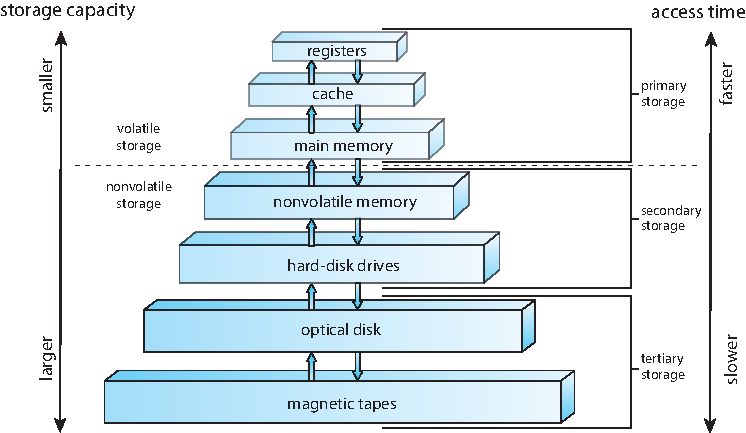
\includegraphics[height = 6cm]{figures/storage_hierarchy.pdf}
    % \caption{} % \label{}
\end{figure}
From here onwards, the term \textbf{memory} will be used to refer to
volatile storage, while \textbf{nonvolatile storage} (NVS) will be
used to refer to nonvolatile storage.

The design of a complete storage system must balance,
\begin{itemize}
    \item Cost: NVS is cheaper than memory
    \item Performance: memory is faster than NVS
    \item Volatility: memory loses its contents when power is lost
\end{itemize}
\subsection{I/O	Structure}
I/O is structured in one of two ways:
\begin{enumerate}
    \item After I/O starts, control returns to the user program only
          upon I/O completion.
          \begin{itemize}
              \item \textbf{Wait instructions} idle the CPU until the
                    next interrupt
              \item At most one I/O request is outstanding at a time,
                    and no simultaneous I/O processing is possible
          \end{itemize}
    \item After I/O starts, control returns to the user program without
          waiting for I/O completion.
          \begin{itemize}
              \item \textbf{System calls} request the OS to allow the
                    user to wait for I/O completion
              \item A \textbf{device-state table} contains entries for
                    each I/O device, indicating its type, address, and
                    state
              \item The OS indexes into this table to determine the
                    device status and modifies the table entry to
                    include interrupt information
          \end{itemize}
\end{enumerate}
\subsubsection{Direct Memory Access}
The form of interrupt-driven I/O described above is sufficient for
moving small amounts of data, but can produce high \textbf{overhead}
when used for bulk data transfer.

To solve this problem, \textbf{direct memory access} (DMA) is used.
This allows device controllers to transfer entire blocks of data
directly to or from the device and main memory, without CPU
intervention. Only one interrupt is generated per block, to indicate
the operation has completed, rather than one interrupt per byte.
\begin{figure}[H]
    \centering
    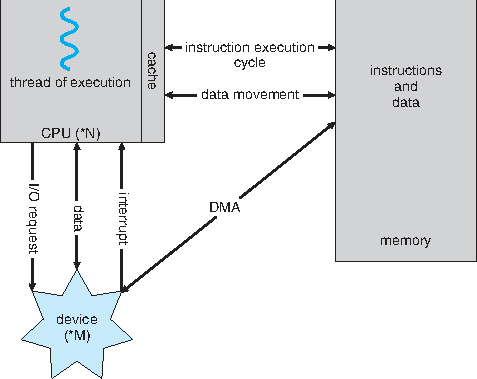
\includegraphics[height = 6cm]{figures/dma.pdf}
    % \caption{} % \label{}
\end{figure}
While the device controller is performing these operations, the CPU is
idle, and can be used by another process.
\subsection{Computer-System Architecture}
\begin{tcolorboxlarge}[title={Definitions}, parbox=false]
    This section will use the following definitions:
    \begin{description}
        \item[Processing Core] The basic computation unit of a CPU
        \item[Central Processing Unit] The hardware that executes
              instructions
        \item[Processor] A physical chip that contains one or more CPUs
        \item[Multicore] A CPU with multiple cores
        \item[Multiprocessor] A system with multiple processors
    \end{description}
\end{tcolorboxlarge}
\subsubsection{Single-Processor Systems}
A single processor system is one which contains a single general
purpose CPU with a single processing core.

Older computer systems used a single processor containing one CPU with
a single processing core. The \textbf{core} is the component that
executes instructions and accesses registers for storing data locally.
The \textbf{CPU} is capable of executing a \textbf{general-purpose}
instruction set, including instructions from processes.

These systems also have other \textbf{special-purpose} processors such
as device-specific processors for disk, keyboard, and graphics
controllers. These processors run a limited instruction set and cannot
run processes.

Sometimes these processors are managed by the OS, which sends them
information about the next task and monitors their status.

In other systems, special-purpose processors are low-level components
built into the hardware. The OS cannot communicate with these
processors, as they execute jobs autonomously.
\subsubsection{Multiprocessor Systems}
Multiprocessor systems (or \textbf{parallel (tightly-coupled)
systems}), are systems with two or more processors.
\begin{figure}[H]
    \centering
    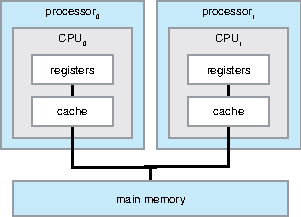
\includegraphics[height = 6cm]{figures/multiprocessing.pdf}
    % \caption{} % \label{}
\end{figure}
Multiprocessor systems have several advantages over single processor
systems:
\begin{itemize}
    \item \textbf{Increased throughput}: More work can be accomplished
          in less time
    \item \textbf{Economy of scale}: Multiprocessor systems are cheaper
          than equivalent multiple single processor systems
    \item \textbf{Increased reliability}: Graceful degradation or fault
          tolerance --- if one CPU fails, the system can continue to
          operate
\end{itemize}
There are two types of multiprocessor systems:
\begin{itemize}
    \item \textbf{Asymmetric multiprocessing}: Each processor is
          assigned a specific task, such as I/O or process scheduling
    \item \textbf{Symmetric multiprocessing}: Each processor performs
          all tasks, including OS activities
\end{itemize}
\begin{tcolorboxlarge}[title={Symmetric Multiprocessing}, parbox=false]
    The most common multiprocessor systems use symmetric multiprocessing
    (SMP), where each CPU performs all tasks, including operating system
    functions and user processes. Each CPU has its own registers and
    cache, but all processors share physical memory over the
    \textbf{same bus}.

    The benefit of this model is that many processes can be run
    \textbf{simultaneously}, without performance degradation. However,
    since CPUs are separate, one may be idle which another is busy,
    resulting in inefficiencies.

    One solution to this problem is to share certain \textbf{data
    structures} between processors. This will allow processors and
    resources (such as memory) to be shared dynamically amongst
    processors, reducing workload variation between processors.

    Such systems must properly \textbf{schedule} and
    \textbf{synchronise} access to shared resources, to avoid conflicts
    between processors.
\end{tcolorboxlarge}

\begin{tcolorboxlarge}[title={Multicore Systems}, parbox=false]
    Multicore systems are systems with multiple computing cores on the
    same chip (processor).
    \begin{figure}[H]
        \centering
        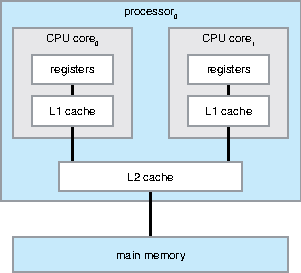
\includegraphics[height = 6cm]{figures/multicore.pdf}
        % \caption{} % \label{}
    \end{figure}
    Multicore systems:
    \begin{itemize}
        \item are more efficient than systems with multiple chips with
              single cores, because on-chip communication is faster
              than between-chip communication.
        \item use significantly less power than multiple single core
              chips.
    \end{itemize}
    Each core has its own local cache, known as \textbf{level-1}, or
    \textbf{L1 cache}.
    In addition to this, each core shares a \textbf{level-2}, or
    \textbf{L2 cache}, that is local to the chip.
    Lower levels of cache are generally smaller, but have faster access
    times than higher level shared caches.

    A multicore processor with \(N\) cores appears to the operating
    system as \(N\) standard CPUs. This requires operating system
    designers and application programmers to make efficient use of
    these additional processing cores.
\end{tcolorboxlarge}
\begin{tcolorboxlarge}[title={Non-Uniform Memory Access Multiprocessing Systems}, parbox=false]
    While adding additional CPUs to multiprocessor systems increases
    computing power, contention for the system bus creates a bottleneck
    and limits performance. An alternative approach is to provide each
    CPU (or groups of CPUs) with its own \textbf{local memory} that is
    accessed via a small but fast, local bus. These CPUs are connected
    by a \textbf{shared system interconnect}, so that all CPUs share one
    physical address space.

    This is known as a \textbf{non-uniform memory access} (NUMA)
    architecture.
    \begin{figure}[H]
        \centering
        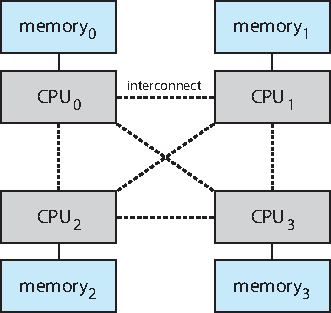
\includegraphics[height = 6cm]{figures/numa.pdf}
        % \caption{} % \label{}
    \end{figure}
    The advantages and disadvantages of NUMA multiprocessing
    architectures are as follows:
    \begin{itemize}
        \item CPUs have fast access to local memory and require no
              contention over the system interconnect
        \item NUMA can be scaled more effectively as more CPUs are
              added
        \item There is increased \textbf{latency} when accessing
              \textbf{remote memory} across the system interconnect
    \end{itemize}
    Due to their excellent scalability, NUMA systems are very popular
    on servers and high-performance computing systems.
\end{tcolorboxlarge}

\begin{tcolorboxlarge}[title={Blade Servers}, parbox=false]
    Blade servers are systems in which multiple processor boards, I/O
    boards, and \linebreak networking boards are placed in the same
    chassis. These servers consist of multiple independent multiprocessor
    systems, that runs its own operating system.
\end{tcolorboxlarge}
\subsubsection{Clustered Systems}
Clustered systems are another type of multiprocessor system that are
composed of two or more individual systems, called \textbf{nodes}. Each
system is typically a multicore system, and the system is
\textbf{loosely coupled}. Clustered computers share storage via a
\textbf{storage-area network} (SAN) and are usually connected via a
\textbf{local-area network} (LAN).
\begin{figure}[H]
    \centering
    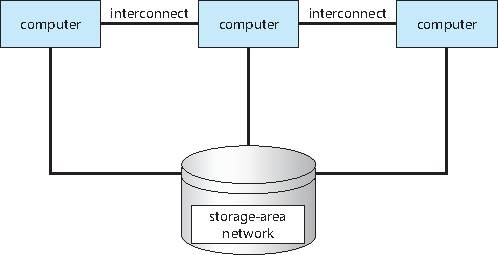
\includegraphics[height = 6cm]{figures/clustered_system.pdf}
    % \caption{} % \label{}
\end{figure}
\begin{tcolorboxlarge}[title={High-Availability Service}, parbox=false]
    The purpose of a clustered system is to provide a \textbf{high
        availability service}, that is,	the ability to operate even if one
    or more nodes fail.	This is achieved by adding a level of redundancy
    in the system. In this system, a layer of cluster software runs on
    the cluster nodes to monitor one or more nodes, such that if the
    monitored machine fails, the monitoring machine can take ownership
    of its resources.

    The ability to continue providing service proportional to the level
    of surviving hardware is called \textbf{graceful degradation}. Some
    systems are called \textbf{fault tolerant} if they can suffer a
    failure of a single component and still continue operation. Fault
    tolerance requires a mechanism to allow the failure to be detected,
    diagnosed, and corrected.

    Clustering can be structured asymmetrically or symmetrically:
    \begin{itemize}
        \item \textbf{Asymmetric clustering} has one
              machine in \textbf{hot-standby mode}, while the other runs
              applications. The hot-standby host machine monitors the
              active server, so that if it fails, it will become the
              active server.
        \item \textbf{Symmetric clustering} has multiple hosts running
              applications, while monitoring each other. This structure
              is more efficient as it uses all available hardware, but
              only if more than one application is running.
    \end{itemize}
\end{tcolorboxlarge}

\begin{tcolorboxlarge}[title={High-Performance Computing}, parbox=false]
    As a cluster consists of several computer systems connected via a
    network, clusters can also provide \textbf{high-performance
        computing} (HPC) environments. Such systems supply significantly
    greater computational power because they can run applications
    concurrently on several computers.

    This is primarily useful for applications that utilise
    \textbf{parallelisation}, which is the process of breaking down a
    large task into smaller components that run on individual cores in
    a computer. These tasks are designed to then be recombined to
    produce the final result.
\end{tcolorboxlarge}

\begin{tcolorboxlarge}[title={Parallel Clustering}, parbox=false]
    Parallel clusters allow multiple hosts to access the same data on a
    shared storage over a \textbf{wide-area network} (WAN).
    Such systems require specialised versions of software that can
    support simultaneous data access by multiple hosts, to ensure that
    no conflicting operations occur.
    This function, commonly known as a \textbf{distributed lock
        manager} (DLM), is included in some cluster technologies.
\end{tcolorboxlarge}
\subsection{Operating System Operations}
\subsubsection{Computer Startup}
When a computer is turned on or rebooted, the first program it runs is
a \textbf{bootstrap program} (\textbf{firmware}), which then loads the
operating system. This program is stored in \textbf{read only memory}
(ROM) or \textbf{electrically erasable programmable read only memory}
(EEPROM). This storage is infrequently written to and is nonvolatile.

This program will search for an operating system kernel within all
connected hard disks, optical drives, or USBs, and load the first one
it finds into memory. The order in which this search is conducted is
known as the \textbf{boot sequence}, and can be configured in the
\textbf{basic input/output system} (BIOS).

Some services are provided outside of the kernel, by system programs,
that are loaded into memory at boot time to become \textbf{system
daemons}, which run while the kernel is running. On Linux, the first
system program is ``\mintinline{text}|systemd|'', and it starts many
other daemons.

Once this is completed, the system is fully booted, and waits for some
event to occur. As discussed earlier, events are signalled via
interrupts.
\subsubsection{Multiprogramming}
Users of a system typically want to run multiple programs at the same
time, rather than having one program keeping the CPU or I/O devices
busy at all times. \textbf{Multiprogramming} allows an operating system
to increase CPU utilisation, and satisfy user requirements, by
organising jobs (code and data) such that the CPU always has one to
execute. In such a system, a program in execution is called a
\textbf{process}.

The operating system keeps a subset of processes in memory, where the
CPU executes processes one at a time, switching between processes when
the current process no longer requires the CPU or is waiting for I/O.
This ensures the CPU is never idle as long as there are processes to
execute. This is known as \textbf{process scheduling}.
\subsubsection{Multitasking}
Multitasking (or \textbf{timesharing}) is a logical extension of
multiprogramming, in which a CPU switches between multiple processes
frequently, providing the illusion that multiple processes are
executing simultaneously. For instance, the time a user takes to type a
command or click a mouse is incredibly slow for a computer, and hence
the CPU may switch to another process while waiting for the user to
provide input.

Multitasked systems require additional considerations:
\begin{itemize}
    \item \textbf{Interactive} systems require fast
          \textbf{response times} (less than 1s), so that
          users do not have to wait for long periods of time.
    \item Having several processes in memory requires \textbf{memory
          management}.
    \item If several processes are ready to be executed, \textbf{CPU
          scheduling} is required to decide which process to execute
          next.
    \item If multiple processes are executing concurrently,
          \textbf{process synchronisation} is required to ensure that
          processes do not interfere with each other.
\end{itemize}
For processes that are larger than \textbf{physical memory},
\textbf{virtual memory} may be used to execute processes that are
stored partially in memory.
This arrangement of memories addresses memory usage constraints.

\emph{Both multiprogramming and multitasking systems must provide a
    \textbf{file system} to allow processes to access data stored on
    secondary storage. In addition to this, they must \textbf{protect
        resources} from inappropriate use, provide mechanisms to process
    \textbf{synchronisation and communication}, and ensure that
    processes do not get stuck in a \textbf{deadlock}.
}
\subsection{Dual-Mode Operation}
As the operating system and users share hardware and software
resources, the operating system must ensure that malicious programs
cannot cause other programs (or the operating system itself) to execute
incorrectly. To distinguish between the execution of operating system
code and user-defined code, we can use \textbf{dual-mode} operation:
\begin{itemize}
    \item \textbf{User mode} --- used for executing
          user-defined code, and restricts direct access to hardware and
          special instructions.
    \item \textbf{Kernel mode} --- used for executing operating system
          code, and allows direct access to hardware and all privileged
          instructions.
\end{itemize}
A \textbf{mode bit} is used to indicate the current mode of operation;
0, when the system is in kernel mode, and 1, when the system is in
user mode.
At system boot time, hardware starts in kernel mode, and the operating
system (when it is loaded), starts user applications in user mode.

When a trap or interrupt occurs, the hardware switches from user mode
to kernel mode, and always switches to user mode \textit{before}
returning control to the user program.

This also allows us to designate certain machine instructions as
\textbf{privileged instructions}, which can only be executed in kernel
mode. For example, the instruction to switch from user mode to kernel
mode is a privileged instruction.

An example is shown in the figure below.
\begin{figure}[H]
    \centering
    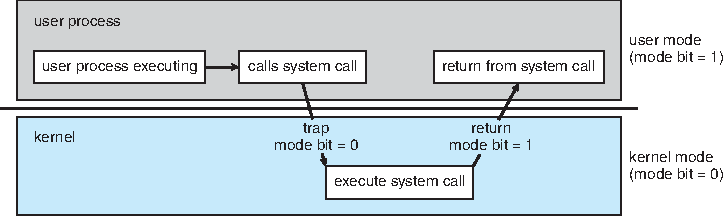
\includegraphics[width = \linewidth]{figures/dual_mode.pdf}
    % \caption{} % \label{}
\end{figure}
\subsection{Multi-Mode Operation}
The dual-mode concept can be extended to include multiple modes of
operation, where each mode has a different level of privilege. One such
example of this is with CPUs that support virtualisation, where a
separate mode is used to indicate when the \textbf{virtual machine
manager} (VMM) is in control of the system.
\subsection{Timers}
To ensure that the operating system maintains control over the CPU, a
\textbf{timer} is used to prevent a user program from running
indefinitely.
\begin{itemize}
    \item The operating system configures a timer to interrupt the CPU
          after a specific period of time, before transferring control
          to the user
    \item The timer is decremented for every clock tick
    \item An interrupt is generated when the timer reaches 0
    \item The operating system decides whether to regain control of the
          CPU, or allow the program to continue running
\end{itemize}
\section{Operating System Structures}
An operating system provides an environment for executing programs and
services to programs and users. One set of operating system services
provides functions that are helpful to the \textbf{user}:
\begin{itemize}
    \item \textbf{User
              interface} --- almost all operating systems have a \textbf{user
              interface} (UI) that is either \textbf{command-line} or
          \textbf{graphical}.
          This interface can be interacted with via the keyboard or
          mouse.
          Touchscreens also provide \textbf{touch screen interfaces}.
    \item \textbf{Program execution} --- The system must be able to load
          programs into memory to run them, and also end their execution,
          either normally, or abnormally (due to an error).
    \item \textbf{I/O operations} --- A running program may require I/O,
          which may involve a file or an I/O device.
          The operating system provides a uniform interface to I/O
          devices.
    \item \textbf{File-system manipulation} --- Programs need to read
          and write files or directories, create or delete them by
          name, search for files, list file information, and manage
          permissions and ownership.
    \item \textbf{Communications} --- Processes may exchange
          information, on the same computer or between computers over a
          network.
          Communications may be via \textbf{shared memory}, in which
          two or more processes read and write to a shared section of
          memory, or through \textbf{message passing}, where packets of
          information in predefined formats are moved between processes
          by the operating system.
    \item \textbf{Error detection} --- The operating system must detect
          and correct errors constantly.
          \begin{itemize}
              \item Errors may occur in the CPU and memory hardware
                    (memory errors or power failures), I/O devices
                    (parity errors or connection failures on a network,
                    or lack of paper in a printer), and in user
                    programs (division by zero or invalid memory
                    access).
              \item The operating system must take the appropriate
                    action to ensure correct and consistent computing.
              \item Debugging facilities can enhance the user's and
                    programmer's abilities to efficiently use the
                    system.
          \end{itemize}
\end{itemize}
Another set of operating system functions exist to ensure efficient
operation of the system via resource sharing:
\begin{itemize}
    \item \textbf{Resource allocation} --- When multiple users or
          multiple jobs running concurrently, resources must be
          allocated to each of them.
          \begin{itemize}
              \item some resources (CPU cycles, main memory, and file
                    storage), may have a special allocation code
              \item others (such as I/O devices) may have general
                    request and release codes
          \end{itemize}
    \item \textbf{Accounting} (\textbf{logging}) --- Keeping track of
          which programs use how much and what kinds of computer
          resources. This is valuable for system administration where a
          system can be fine-tuned to improve performance.
    \item \textbf{Protection and security} --- The owners of information
          stored in a multi-user or networked system must be able to
          control access to that information.
          \begin{itemize}
              \item Concurrent processes should not interfere with each
                    other or the operating system itself
              \item \textbf{Protection} ensures that all access to
                    system resources is controlled
              \item \textbf{Security} requires authentication from
                    external users. This extends to defending external
                    I/O devices from invalid access attempts
              \item If a system is to be protected and secure,
                    precautions must be instituted throughout it. A
                    chain is only as strong as its weakest link.
          \end{itemize}
\end{itemize}
\subsection{User and Operating System Interface}
There are many ways for users to interface with the operating system.
\subsubsection{Command Interpreters}
Most operating systems, including, Linux, UNIX, and Windows, treat
command interpreters as a \textbf{special program} that is running when
a process is initiated. On systems with multiple command interpreters,
these are known as \textbf{shells}.

For example, on UNIX and Linux systems, users may choose among several
shells including the \textbf{C shell}, \textbf{Bourne-Again shell},
\textbf{Korn shell}, and others.

The main function of a command interpreter is to fetch and execute
user-specified commands. These commands can be implemented in two
general ways:
\begin{itemize}
    \item \textbf{Built-in commands} --- Commands that are interpreted
          directly by the command interpreter and do not require the
          execution of another program.
    \item \textbf{System programs} --- The command interpreter does not
          understand the command, and uses the command to identify a file
          to be loaded into memory and executed.
\end{itemize}
If the latter, adding new commands to the system is as simple as
writing a new program, and modifying existing programs does not
require shell modification.
\subsubsection{Graphical User Interface}
Rather than entering commands directly via a command-line interface,
users can use the mouse, keyboard, and monitor to interact with images
and icons on the screen (the desktop). Clicking mouse buttons may
invoke additional actions that can provide information, display
options, execute functions, open directories (folders), and so on.

Many systems now include both a CLI and GUI:
\begin{itemize}
    \item \textbf{macOS} is implemented on the UNIX kernel, and provides
          an \textit{Aqua} GUI and a command-line interface
    \item \textbf{Windows} provides a standard GUI and a CLI
    \item \textbf{UNIX and Linux} provide CLI shells with optional GUIs
          such as \textit{K Desktop Environment} (KDE), or the GNOME
          desktop by the GNU project.
\end{itemize}
\subsubsection{Touch Screen Interface}
As a command-line or mouse-and-keyboard system is impractical for
mobile systems, phones, tablets, and other mobile devices use a touch
screen interface. These devices require the user to interact with the
screen directly using gestures and a virtual keyboard.
\subsection{System Calls}
System calls provide an interface to the services made available by an
operating system. These calls are generally available as functions
written in C and C++, or sometimes Assembly.

These functions are typically accessed via a high-level
\textbf{application programming interface} (API), rather than direct
system calls.

Observe the following example of a system call sequence where we wish
to copy a file's contents into another file:
\begin{minted}{text}
Acquire input file name
  Write prompt to screen
  Accept input
Acquire output file name
  Write prompt to screen
  Accept input
Open the input file
  if file doesn't exist, abort
Create output file
  if file exists, abort
Loop
  Read from input file
  Write to output file
Until read fails
Close output file
Write completion message to screen
Terminate normally
\end{minted}
\subsection{Application Programming Interface}
Even a simple program makes heavy use of the operating system. For this
reason, application programmers design programs according to an
\textbf{application programming interface} (API). This API specifies a
set of functions that are available to an application programmer,
including the parameters that are passed to each function and the
return values the programmer can expect. On UNIX systems, we can use
the \mintinline{text}|man| command to view the API for a given
function.

Some examples of APIs include:
\begin{itemize}
    \item the \textbf{Windows API} for Windows systems
    \item the \textbf{POSIX API} for UNIX, Linux, and macOS
\end{itemize}
A programmer accesses an API via a \textbf{library} of code, provided by
the operating system.
In the case of UNIX and Linux, programs written in the C language use a
library called \textbf{libc}.

There are two main reasons for programming according to an API:
\begin{itemize}
    \item \textbf{Program portability} --- a program written to an API
          can be compiled on any system that supports that API
    \item \textbf{Ease of implementation} --- making system
          calls manually may require more work and a deeper
          understanding of system functions
\end{itemize}
\subsubsection{System Call Interface}
An important factor in handling system calls is the \textbf{run-time
environment} (RTE), which is a suite of software needed to execute
applications written in a particular programming language, including
compilers, interpreters, libraries and loaders. The RTE provides a
\textbf{system-call interface} that serves as a link to system calls
made available by the operating system.

The system-call interface \textbf{intercepts} function calls in the API
and invokes the necessary system calls within the operating system.
Typically a number is associated with each system call, and the
system-call interface maintains a table indexed according to these
numbers. The system-call interface invokes the intended system call in
the operating system kernel and returns the status of the system call
with any return values.

Thus, the caller does not need to know anything about how the system
call is implemented, rather it only needs to know obey the API and
understand what the operating system will do as a result of this call.
Below is an example of a user application invoking the
\mintinline{text}|open()| system call:
\begin{figure}[H] \centering
    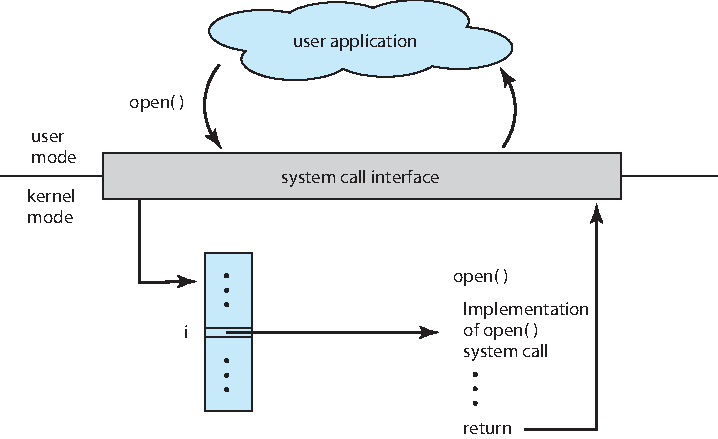
\includegraphics[height = 6cm]{figures/system_call_open.pdf}
    % \caption{} % \label{}
\end{figure}
\subsubsection{System Call Parameter Passing}
Often more information is required than simply the identity of the
desired system call. There are three general methods used to pass
parameters to the operating system:
\begin{itemize}
    \item \textbf{Registers} --- pass parameters to registers
    \item \textbf{Blocks} --- parameters are stored in a block, or
          table, in memory, and the address of the block is passed as a
          parameter in a register
    \item \textbf{Stack} --- parameters are pushed onto the stack, and
          popped by the operating system
\end{itemize}
The latter two approaches are preferred as they do not limit the number
or length of parameters being passed.
\begin{figure}[H]
    \centering
    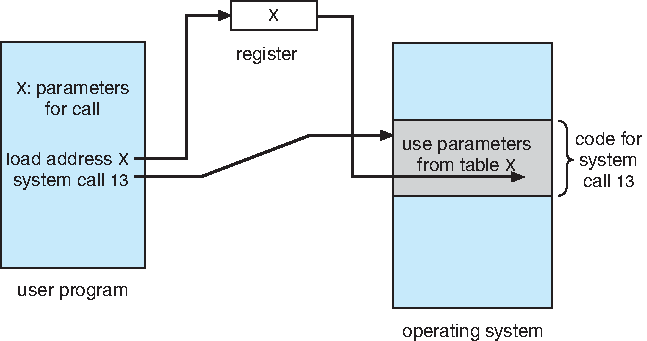
\includegraphics[height = 6cm]{figures/system_call_param_pass.pdf}
    % \caption{} % \label{}
\end{figure}
\subsection{Types of System Calls}
System calls can be grouped into six major categories:
\begin{itemize}
    \item Process control
    \item File management
    \item Device management
    \item Information maintenance
    \item Communications
    \item Protection
\end{itemize}
Some examples of these types of system calls are shown
in the following sections.
\subsubsection{Process Control}
% A running program needs to be able to halt its execution either normally (\mintinline{text}|end()|)
% or abnormally (\mintinline{text}|abort()|). If a system call is made to terminate a program abnormally,
% or if the program causes an error trap, an error is displayed, and a dump of memory is written
% to a special log file on disk to be examined by a \textbf{debugger}, which is a system program designed
% to aid the programmer in finding and correcting \textbf{bugs}.

% Some systems may allow for special recovery actions by defining an error level. More severe errors can
% be indicated by a higher-level error parameter. Normal termination can then be defined as an error at
% level 0. The command interpreter can use this error level to determine the next action automatically.

% A process may wish to load or execute another program, which can be achieved via the \mintinline{text}|exec()|

% Summary of process control system calls:
\begin{itemize}
    \item create process, terminate process
    \item load, execute
    \item get process attributes, set process attributes
    \item wait event, signal event
    \item allocate and free memory
\end{itemize}
\subsubsection{File Management}
\begin{itemize}
    \item create file, delete file
    \item open, close
    \item read, write, reposition
    \item get file attributes, set file attributes
\end{itemize}
\subsubsection{Device Management}
\begin{itemize}
    \item request device, release device
    \item read, write, reposition
    \item get device attributes, set device attributes
    \item logically attach or detach devices
\end{itemize}
\subsubsection{Information Maintenance}
\begin{itemize}
    \item get time or date, set time or date
    \item get system data, set system data
    \item get process, file, or device attributes
    \item set process, file, or device attributes
\end{itemize}
\subsubsection{Communications}
\begin{itemize}
    \item create, delete communication connection
    \item send, receive messages
    \item transfer status information
    \item attach or detach remote devices
\end{itemize}
\subsubsection{Protection}
\begin{itemize}
    \item get file permissions
    \item set file permissions
\end{itemize}
\subsubsection{Examples of Windows and UNIX System Calls}
\begin{table}[H]
    \centering
    \begin{tabular}{l c c}
        \toprule
                                                          & \textbf{Windows}                                  & \textbf{UNIX}                 \\
        \midrule
        \multirow{3}{*}{\textbf{Process Control}}         & \mintinline{text}|CreateProcess()|                & \mintinline{text}|fork()|     \\
                                                          & \mintinline{text}|ExitProcess()|                  & \mintinline{text}|exit()|     \\
                                                          & \mintinline{text}|WaitForSingleObject()|          & \mintinline{text}|wait()|     \\[1em]

        \multirow{4}{*}{\textbf{File Management}}         & \mintinline{text}|CreateFile()|                   & \mintinline{text}|open()|     \\
                                                          & \mintinline{text}|ReadFile()|                     & \mintinline{text}|read()|     \\
                                                          & \mintinline{text}|WriteFile()|                    & \mintinline{text}|write()|    \\
                                                          & \mintinline{text}|CloseHandle()|                  & \mintinline{text}|close()|    \\[1em]

        \multirow{3}{*}{\textbf{Device Management}}       & \mintinline{text}|SetConsoleMode()|               & \mintinline{text}|ioctl()|    \\
                                                          & \mintinline{text}|ReadConsole()|                  & \mintinline{text}|read()|     \\
                                                          & \mintinline{text}|WriteConsole()|                 & \mintinline{text}|write()|    \\[1em]

        \multirow{3}{*}{\textbf{Information Maintenance}} & \mintinline{text}|GetCurrentProcessID()|          & \mintinline{text}|getpid()|   \\
                                                          & \mintinline{text}|SetTimer()|                     & \mintinline{text}|alarm()|    \\
                                                          & \mintinline{text}|Sleep()|                        & \mintinline{text}|sleep()|    \\[1em]

        \multirow{3}{*}{\textbf{Communications}}          & \mintinline{text}|CreatePipe()|                   & \mintinline{text}|pipe()|     \\
                                                          & \mintinline{text}|CreateFileMapping()|            & \mintinline{text}|shm_open()| \\
                                                          & \mintinline{text}|MapViewOfFile()|                & \mintinline{text}|mmap()|     \\[1em]

        \multirow{3}{*}{\textbf{Protection}}              & \mintinline{text}|SetFileSecurity()|              & \mintinline{text}|chmod()|    \\
                                                          & \mintinline{text}|InitializeSecurityDescriptor()| & \mintinline{text}|umask()|    \\
                                                          & \mintinline{text}|SetSecurityDescriptorGroup()|   & \mintinline{text}|chown()|    \\
        \bottomrule
    \end{tabular}
    % \caption{} % \label{}
\end{table}
\subsection{System Services}
System services, also known as system programs or utilities, provide a
convenient environment for program development and execution. Some are
simply user interfaces to system calls, while others are considerably
more complex. Most users' view of the operating system is defined by
system programs, not the actual system calls.
\begin{itemize}
    \item \textbf{File management}.
          Programs that create, delete, copy, rename, print, list, or
          access and manipulate, files and directories.
    \item \textbf{Status information}.
          Programs that ask the system for the date, time, amount of
          available memory or disk space, number of users, or similar
          status information.
          Other programs provide detailed performance, logging, and
          debugging information.
          This information is typically formatted and outputted to the
          user.

          Some systems also support a \textbf{registry}, which is used
          to store and retrieve configuration information.
    \item \textbf{File modification}.
          Text editors may create and modify the content of files
          stored on disk.
          There may be special commands to search files or perform
          transformations of the text.
    \item \textbf{Programming-language support}.
          Compilers, assemblers, debuggers, and interpreters for common
          programming languages (such as C, C++, Java, and Python) are
          often provided with the operating system or available to
          download.
    \item \textbf{Program loading and execution}.
          Once a program is assembled or compiled, it must be loaded
          into memory to be executed.
          The system may provide absolute loaders, relocatable loaders,
          linkage editors, and overlay loaders.

          Debugging systems for either higher-level languages or
          machine language are needed as well.
    \item \textbf{Communications}.
          These programs provide the mechanism for creating virtual
          connections among processes, users, and computer systems.
          They also allow users to send information to other machines.
    \item \textbf{Background services}.
          All general-purpose systems have methods for launching
          certain system-program processes at boot time.
          Some of these processes terminate after completing their
          tasks, while others continue to run until the system is
          halted.
          Constantly running processes are called services, subsystems,
          or daemons.
\end{itemize}
Along with these system programs, most operating systems are supplied
with application programs that are designed to perform common
operations.
\subsection{Operating System Design and Implementation}
\subsubsection{Mechanisms and Policies}
An important principle is the separation of \textbf{policy} from
\textbf{mechanism}. Policies determine \textit{what} will be done, and
mechanisms determine \textit{how} to do something.

The separation of policy and mechanism is important for
\textbf{flexibility}. Policies are likely to change over time, and
should not require a change in the underlying mechanism.

Microkernel based systems take this principle to the extreme, by only
implementing a basic set of policy-free building blocks, so that more
advanced mechanisms and policies can be added via user-created kernel
modules.

In contrast, the Windows operating system and macOS, closely encode
both mechanism and policy into the system to enforce a global look and
feel across the system. All applications will therefore have similar
interfaces, because the interface itself is built into the kernel and
system libraries.
\subsubsection{Implementation}
Operating systems are typically implemented using several
\textbf{high-level languages} such as C, C++, and assembly. While the
kernel might be written assembly and C, higher-level routines and
system libraries may be written using C++.

Some reasons for using higher-level languages are described below:
\begin{itemize}
    \item Code is faster to write
    \item Code is more compact
    \item Code is easier to understand
    \item Code is easier to debug
\end{itemize}
In addition to this,
improvements in compiler technology will improve the
generated code for the entire operating system.

Another advantage is that operating systems can be \textbf{ported} to
other hardware if they are written in a higher-level language. This is
particularly important for operating systems intended to run on
different hardware systems, such as embedded devices, Intel x86
systems, and ARM chips in mobile devices.
\subsection{Operating System Structure}
A system as large and complex as an operating system must be engineered
carefully if it is to function properly and be modified easily. We will
discuss the evolution of various structures in the following sections.
\subsubsection{Monolithic Structures}
The monolithic structure is the \textbf{simplest} structure for
organising an operating system, as it uses \textbf{no structure} at
all. All functionality of the kernel is placed into a single, static
binary file, that runs in a single address space.

An example of such a structure is the original UNIX operating system,
which consists of two separable parts:
\begin{itemize}
    \item the kernel
    \item system programs
\end{itemize}
The kernel represents everything \underline{below the system-call
    interface} and \underline{above the physical hardware}.
It provides the file system, CPU scheduling, memory management, and
other operating-system functions through system calls.
\begin{figure}[H]
    \centering
    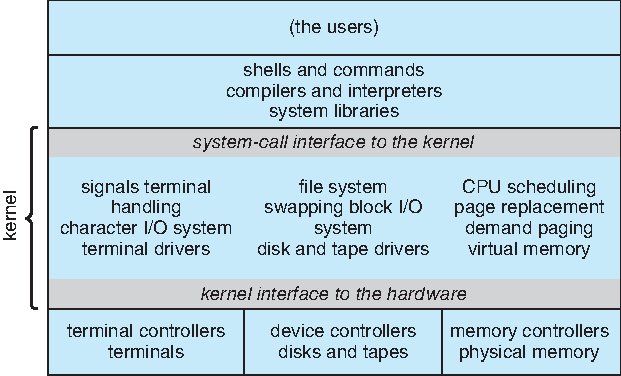
\includegraphics[height = 6cm]{figures/UNIX_structure.pdf}
    % \caption{} % \label{}
\end{figure}
The Linux operating system is based on UNIX and is structured
similarly.
Applications typically use the \mintinline{text}|glibc| standard C
library when communicating with the kernel (through the system-call
interface).
The Linux kernel is monolithic, but has a \textbf{modular design} that
allows the kernel to be modified during runtime.
\begin{figure}[H]
    \centering
    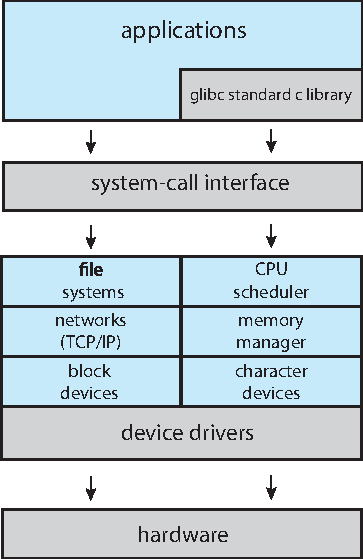
\includegraphics[height = 6cm]{figures/linux_structure.pdf}
    % \caption{} % \label{}
\end{figure}
Monolithic kernels introduce very little overhead in the system-call
interface, and communication within the kernel is very fast.
Despite their simplicity, monolithic kernels are however difficult to
implement and extend.
\subsubsection{Layered Structures}
The monolithic approach is a \textbf{tightly coupled} system because
changes to one part of the system have widespread effects on other
parts of the system. Alternatively, we may consider a \textbf{loosely
coupled} system which is divided into separate, smaller components that
have specific and limited functionality. All these components comprise
the kernel.

One way to achieve modularity is to use a \textbf{layered approach},
where the operating system is divided into a number of layers (levels).
The bottom layer (layer 0) is the hardware, and the highest (layer N)
is the user interface. This is shown below.
\begin{figure}[H]
    \centering
    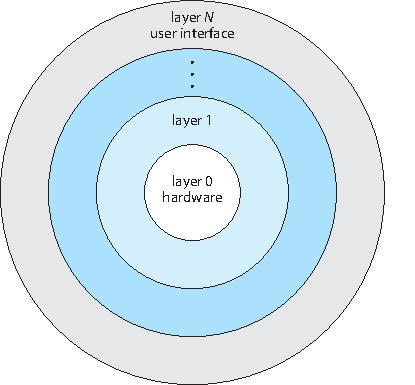
\includegraphics[height = 6cm]{figures/layered_structure.pdf}
    % \caption{} % \label{}
\end{figure}
Each layer uses functions (operations) and services of only
\textbf{lower-level layers}.
This simplifies debugging and system verification.

Layered systems are used in computer networks (such as TCP/IP) and web
applications, however relatively few operating systems use a purely
layered approach due to the challenges of appropriately defining the
functionality of each layer.
\subsubsection{Microkernel Structures}
As UNIX expanded, the kernel became large and difficult to manage, and
thus a system called \textbf{Mach} was developed to modularise the
kernel using the \textbf{microkernel} approach. The Mac OS X kernel,
Darwin, is a well-known example of a microkernel operating system based
on Mach.

In a microkernel structure, \textbf{all nonessential components} are
removed from the kernel and are instead implemented as
\textbf{user-level programs} that reside in separate address spaces.
Typically, microkernels provide minimal process and memory management,
in addition to a communication facility, resulting in a small (micro)
kernel.

The main function of the microkernel is to provide communication
between the client program and the various services that are also
running in user space, using \textbf{message passing}.

There are several benefits of using a microkernel system:
\begin{itemize}
    \item Easy to extend --- new services added to the user space
          rarely require modification to the kernel. Changes to the
          kernel are also smaller
    \item Easy to port to new architectures
    \item More reliable and secure --- most services are running as
          user processes, rather than kernel processes
\end{itemize}
One of the main disadvantages of
microkernels is the \textbf{performance overhead} associated
with user space to kernel space communication.
Communication between two user processes requires messages to be copied
twice; once from the sending process to the kernel, and again from the
kernel to the receiving process.
\begin{figure}[H]
    \centering
    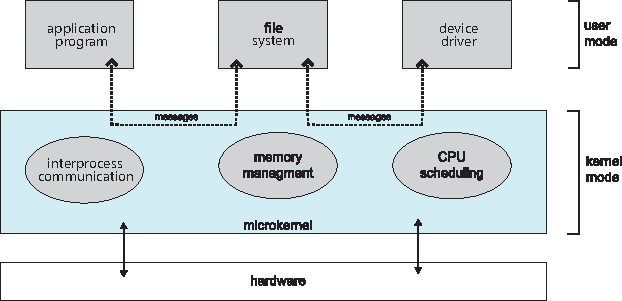
\includegraphics[height = 6cm]{figures/microkernel_structure.pdf}
    % \caption{} % \label{}
\end{figure}
\subsubsection{Modules}
Most modern operating systems use \textbf{loadable kernel modules}
(LKMs). Here, the kernel has a set of core components and can link in
additional services via modules, either at boot time, or during run
time. This design is common to modern implementatios of UNIX, such as
Linux, macOS, and Solaris, and also Windows.

In this structure, the kernel only provides core services, while other
services are implemented \textbf{dynamically}, as the kernel is
running. Linking services dynamically is preferable to adding new
features directly to the kernel, as the latter requires recompiling the
kernel every time a change is made.

The overall result resembles a layered system as each kernel section
has defined, protected interfaces; however, it is more flexible than a
layered system, as any module can call any other module.

This approach is also similar to the microkernel approach in that the
primary module has only core functions and knowledge of how to load and
communicate with other modules; but it is more efficient as modules do
not need to invoke message passing in order to communicate.

Linux uses loadable kernel modules, primarily for device drivers. LKMs
can be ``inserted'' into the kernel as the system is \textbf{booted} or
during run time. If a device is not present, it can be dynamically
loaded.
\subsubsection{Hybrid Structures}
Most modern systems combine several of the above approaches, resulting
in hybrid systems that address performance, security, and usability
issues. For example,
\begin{itemize}
    \item Linux is monolithic to provide performance, and modular to
          allow dynamic loading of kernel services
    \item Windows is also monotlithic, but retains the behaviour of a
          microkernel system, including support for separate subsystem
          \textit{personalities} that run as user-mode processes
    \item Mac OS X is based on the Mach microkernel, and includes
          dynamically loadable modules called \textbf{kernel
          extensions}
\end{itemize}
\section{Processes}
A \textbf{process} is a program in execution, and is the unit of work
in a modern computing system. Processes need resources to accomplish
their task, including CPU time, memory, files, and I/O devices. These
are typically allocated to processes while it is executing.

Modern operating systems support processes having multiple
\textbf{threads} of control. On systems with multiple hardware
processing cores, these threads can run in \textbf{parallel}. An
important aspect of an operating system is how it \textbf{schedules}
threads onto available processing cores.
\subsection{Process Concept}
Early computers were batch systems that executed \textbf{jobs},
followed by time-shared systems that ran \textbf{user programs} or
\textbf{tasks}. On single-user systems, a user may be able to run
several programs at one time, and even if that is not possible, the
operating system may need to support internal programmed activities,
such as memory management. Thus, the concept of a \textbf{process} was
introduced to encapsulate these activities.
\subsubsection{The Process}
A process is a program in execution. The status of the current activity
of a process is represented by the value of the \textbf{prorgam
counter} and the contents of a processor's registers. The memory layout
of a process is divided into multiple sections, as shown in the figure
below.
\begin{figure}[H]
    \centering
    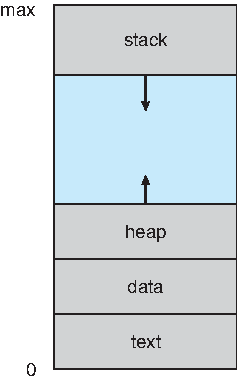
\includegraphics[height = 6cm]{figures/process_memory_layout.pdf}
    % \caption{} % \label{}
\end{figure}
To summarise, these sections include:
\begin{itemize}
    \item \textbf{Text} --- the executable code
    \item \textbf{Data} --- global variables
    \item \textbf{Heap} --- memory dynamically allocated during run time
    \item \textbf{Stack} --- temporary data storage such as function
          parameters, return addresses, and local variables
\end{itemize}
Notice how the sizes of the text and data sections are
\textbf{fixed}, while the sizes of the heap and stack sections may
\textbf{shrink and grow dynamically} during program execution.

When a function is called, an \textbf{activation record} containing
function parameters, local variables, and the return address is pushed
onto the stack. When control is returned from the function, this
activation record is popped off the stack. Similarly, the heap will
grow as memory is dynamically allocated, and will shrink when memory is
returned to the system.

The operating system must ensure that the stack and heap do not
\textbf{overlap} in memory.

It is important to note that a program itself is not a process, but
rather a \textbf{passive entity}, such as an \textbf{executable file},
that contains a list of instructions stored on disk. A process is an
\textbf{active entity} with a program counter specifying the next
instruction to execute, and a set of associated resources.

A \textbf{program} \textit{becomes} a process when an executable file
is loaded into memory, either through a GUI (i.e., mouse double-click),
or through a command line interface. While \textbf{multiple processes}
may be associated with the \textbf{same program}, these are considered
as \textbf{separate} execution sequences, as they may have different
data, heap, and stack sections. A process may also \textbf{spawn} many
other processes as it runs.
\subsubsection{Process State}
As a process executes, it changes \textbf{state} according to its
current activity:
\begin{itemize}
    \item \textbf{New} --- the process is being created
    \item \textbf{Running} --- instructions are being executed
    \item \textbf{Waiting} --- the process is waiting for some event to
          occur (such as an I/O completion or reception of a signal)
    \item \textbf{Ready} --- the process is waiting to be assigned to a
          processor
    \item \textbf{Terminated} --- the process has finished execution
\end{itemize}
It is important to realise that only one
process can be \textbf{running} on any processor at any instant.
A state diagram corresponding to these states is shown below:
\begin{figure}[H]
    \centering
    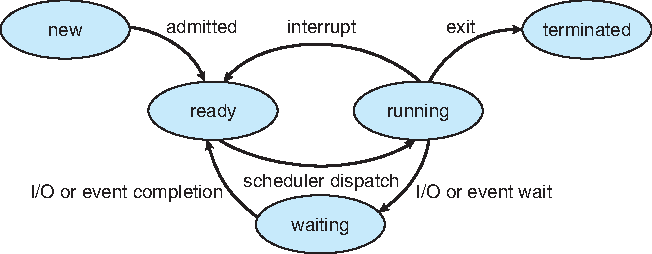
\includegraphics[height = 4cm]{figures/process_state_diagram.pdf}
    % \caption{} % \label{}
\end{figure}
\subsubsection{Process Control Block}
Each process is represented in the operating system by a
\textbf{process control block} (PCB) (also called a \textbf{task
control block}). It contains many pieces of information associated with
a specific process, including:
\begin{itemize}
    \item \textbf{Process state} --- new, ready, running, waiting, halted
    \item \textbf{Program counter} --- the address of the next
          instruction to be executed
    \item \textbf{CPU registers} --- contents of all process-centric
          registers (accumulators, index registers, stack pointers, etc.)
    \item \textbf{CPU-scheduling information} --- process priority, pointers to scheduling queues, etc.
    \item \textbf{Memory-management information} --- memory allocated to the process: base and limit registers, page tables, segment tables
    \item \textbf{Accounting information} --- amount of CPU and real time used, time limits, account numbers, job or process numbers, etc.
    \item \textbf{I/O status information} --- devices allocated to the process, list of open files, etc.
\end{itemize}
To summarise, the PCB serves as the \textbf{repository} for all
information needed to start, or restart, a process.
\subsubsection{Threads}
The process model described above implies that a process is a program
that performs a \textbf{single thread of execution}. This single thread
of control allows the process to perform only one task at a time. Most
modern operating systems have extended the process model to allow a
process to have multiple threads of execution, and thus perform more
than one task at a time. This is especially beneficial on multicore
systems, where multiple threads can run in parallel. On such systems,
the PCB is expanded to include information for each thread.
\subsubsection{Process Representation in Linux}
In Linux, a process is represented by a \mintinline{text}|task_struct|
structure, which is defined in the \mintinline{text}|<linux/sched.h>|
header file. This structure contains a large number of fields,
including:
\begin{minted}{c}
long state;                 /* state of the process */
struct sched entity se;     /* scheduling information */
struct task struct *parent; /* this process’s parent */
struct list head children;  /* this process’s children */
struct files struct *files; /* list of open files */
struct mm struct *mm;       /* address space */
\end{minted}
\subsection{Process Scheduling}
The objective of \textbf{multiprogramming} is to have some process
running at all times, to maximise CPU utilisation. The objective of
\textbf{time sharing} is to switch a CPU core among processes so
frequently that users can interact with each program while it is
running.

To meet these objectives, the \textbf{process scheduler} select an
available process for execution on a core. Each CPU core runs one
process at a time. If there are more processes than cores, the
scheduler must wait until a core is free and can be rescheduled. The
number of processes currently in memory is known as \textbf{degree of
multiprogramming}

Balancing these objectives requires taking the general behaviour of the
process into account.
\begin{itemize}
    \item A process that spends more time doing I/O, is an \textbf{I/O
          bound process}
    \item A process that spends more time doing computation, is an
          \textbf{CPU bound process}
\end{itemize}
\subsubsection{Scheduling Queues}
The process scheduler maintains a set of \textbf{scheduling queues} for
processes awaiting allocation of CPU time. These queues are typically
implemented as \textbf{linked lists} of PCBs, with each queue having
its own priority.
\begin{figure}[H]
    \centering
    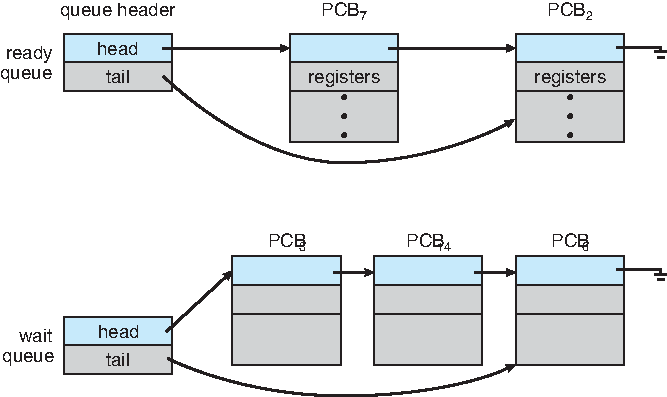
\includegraphics[height = 6cm]{figures/scheduler_queues.pdf}
    % \caption{} % \label{}
\end{figure}
These queues include:
\begin{itemize}
    \item \textbf{Job queue} --- The set of \textbf{all} processes in the system
    \item \textbf{Ready queue} --- As processes enter the system, they
          are placed in this queue which resides in main memory, where
          they are ready and waiting to execute
    \item \textbf{Wait queue} --- The set of processes waiting for the
          occurrenece of an event, such as I/O completion
\end{itemize}
Processes are initially placed in the \textbf{ready queue} where they
wait to be selected by scheduler, or are \textbf{dispatched}.
When a processes is allocated to a CPU core, and is executing, one of
several events may occur:
\begin{itemize}
    \item The process may issue an I/O request and be placed in the
          \textit{wait queue}
    \item The process may create a new child process and be placed in
          the \textit{wait queue} while awaiting the child's
          termination
    \item The process may be removed forcibly from the CPU by the
          scheduler, either due to an interrupt or because that
          process's time slice has expired, and be placed back in the
          \textit{ready queue}
\end{itemize}
In the first two cases, the process eventually returns to the ready queue.
A process continutes this cycle until it terminates, at which point, it
is removed from all queues and has its PCB and resources deallocated.

This is shown in the queueing diagram below:
\begin{figure}[H]
    \centering
    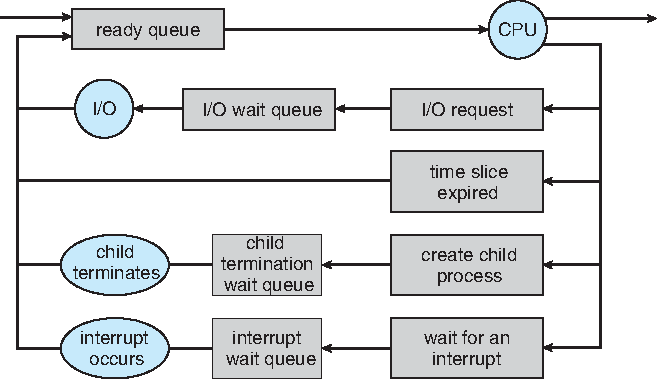
\includegraphics[height = 6cm]{figures/queueing_diagram}
    % \caption{} % \label{}
\end{figure}
\subsubsection{CPU Scheduling}
Processes migrate between the ready and wait queues throughout their
lifetimes. The role of the \textbf{CPU scheduler} is to select from
among the processes that are in the ready queue, and allocate a CPU
core to one of them. This is known as \textbf{CPU scheduling}.

These schedulers are invoked at a different rate,
\begin{itemize}
    \item The process scheduler is a \textbf{long-term scheduler}, as
          it is not invoked very frequently (seconds to minutes).
    \item The CPU scheduler is a \textbf{short-term scheduler}, as it
          is invoked frequently to prevent a single process from using
          a core for an extended period of time. The CPU scheduler
          often forcibly removes the CPU from a process every 100ms or
          faster.
\end{itemize}
Some operating systems have an intermediate form of scheduling known
as \textbf{swapping}.
This is a form of \textbf{medium-term scheduling}, where a process is
removed from memory to reduce the degree of multiprogramming.
This process can be reintroduced into memory later.
A processes state is ``swapped-out'' from memory to disk, where its
current status is saved, and later ``swapped-in'' to memory, with its
status restored.
This is useful when memory has been overcommitted and needs to be freed
up.
\subsubsection{Context Switch}
When the CPU switches to another process, the kernel performs a
\textbf{state save} of the \textbf{current context} of the running
process, then perform a \textbf{state restore} of that context when
processing is complete. The \textbf{context} of a process is
represented in the PCB of that process.

This process is known as a \textbf{context switch}.
\begin{figure}[H]
    \centering
    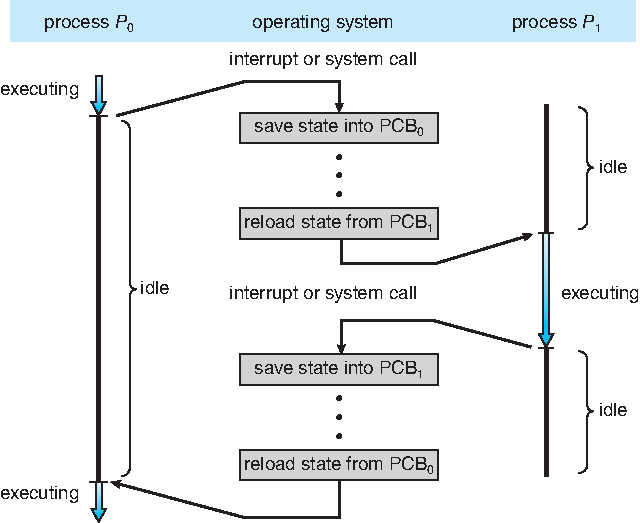
\includegraphics[height = 6cm]{figures/context_switching.pdf}
    % \caption{} % \label{}
\end{figure}
Context switch time is pure overhead, as the system does no useful
work while switching.
More complex operating systems may require more information to be
stored during a context switch, requiring more advanced
memory-management techniques to be implemented.
\subsection{Operations on Processes}
The processes in most systems can execute concurrently, and may be
created and deleted dynamically. These systems must provide a mechanism
for process creation and termination.
\subsubsection{Process Creation}
During execution, a process may create several new processes. The
creating process is called the \textbf{parent process} and the new
processes are known as \textbf{child processes}. Each of these new
processes may in turn create other processes, forming a \textbf{tree}
of processes.

Most operating systems (including UNIX, Linux, and Windows) identify
processes using a \textbf{process identifier} (pid), represented by an
integer. The pid is unique for each process in the system, and can be
used as an index to access various attributes of a process within the
kernel.

In Linux, the \mintinline{text}|systemd| process is the first process
to be created, and has a pid of 1. This process is responsible for
starting all other processes in the system, such as the
\mintinline{text}|logind| and \mintinline{text}|sshd| processes.
\begin{figure}[H]
    \centering
    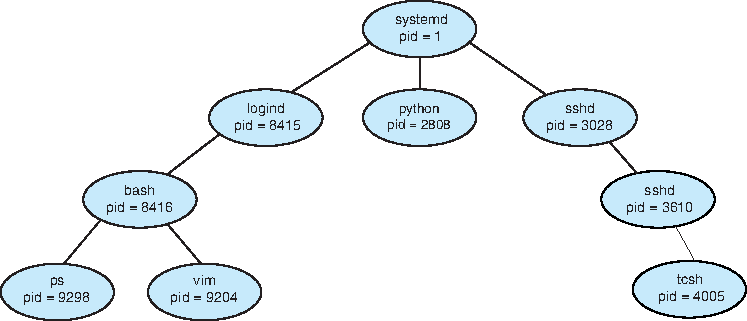
\includegraphics[height = 6cm]{figures/linux_process_tree.pdf}
    % \caption{} % \label{}
\end{figure}
In general, when a process creates a child process, the child will
need certain resources to accomplish its task.
This process may be able to obtain these resources directly from the
operating system, or be constrained to a subset of the parent's
resources.
In addition to supplying physical and logical resources, the parent
process may pass initialisation data (input) to the child process.

When a process creates a new process, two possibilities for execution
exist:
\begin{itemize}
    \item The parent continues to execute concurrently with its
          children
    \item The parent waits until some or all of its children have
          terminated
\end{itemize}
There are also two address-space possibilites for
the new process:
\begin{itemize}
    \item The child process is a duplicate of the parent process (both
          share the same data)
    \item The child process has a new program loaded into it
\end{itemize}
In UNIX,
the \mintinline{text}|fork()| system call is used to
duplicate the calling process and create a new
process.
This allows the parent process to easily communicate with its child
process.
The child may then use the \mintinline{text}|exec()| system call to
replace its memory space with a new program.

The parent process can either create more children, or issue a
\mintinline{text}|wait()| system call to wait for a child to terminate.

When the \mintinline{text}|fork()| system call is invoked, the function
returns the child processes pid to the parent process, but returns 0 to
the child process. This allows us to distinguish between the parent and
child process.

Consider the following code: \inputminted{c}{code/create_process.c}
This program forks the parent process on line 11, and then waits for
the child process to terminate. This program outputs the following:
\begin{minted}{text}
Child:  fork() returned     0 PID 15515
create_process.c  create_process
Parent: fork() returned 15515 PID 15514
\end{minted}
After the child process is created, the
\mintinline{text}|exec()|\footnote{Note that \mintinline{text}|exec()|
is often used to refer to a family of functions in C. While these
functions refer to the same system call, they differ in the arguments
they can accept. See the manpage for \mintinline{text}|exec| for more
information.} system call is used to replace the child's memory space
with the \mintinline{text}|ls| program, causing the second print
statement to not be executed.

The parent process can use the \mintinline{text}|wait()| system call to
remove itself from the ready queue until the termination of the child
process, after which the parent process can resume from where it left
off.
\subsubsection{Process Termination}
A process terminates when it finishes executing its final statement,
and asks the operating system to delete it by using the
\mintinline{text}|exit()| system call. At this point, the process may
return a status value to its parent, which is used to determine if the
child process completed successfully. All resources allocated to the
process are then deallocated and reclaimed by the operating system.

A parent may terminate the execution of one or more of its children by
using the \mintinline{text}|abort()| system call. This may be done for
several reasons, including:
\begin{itemize}
    \item The child process exceeded allocated resources
    \item The task assigned to the child is no longer required
    \item The parent is exiting, and the operating system does not
          allow a child to continue if its parent terminates. As a
          result, all child processes are terminated ---
          \textbf{cascading termination}
\end{itemize}
The following
example demonstrates how a parent process might see the exit
status of a child process.
\inputminted{c}{code/terminate_process.c}
This program outputs the following:
\begin{minted}{text}
Child PID 28453
PID 28453 exited with status 0x100
Exit code: 1
\end{minted}
When a process terminates, its resources are deallocated by the
operating system. However, its entry in the process table must remain
until the parent calls \mintinline{text}|wait()|, because the process
table contains the process's exit status.
\begin{itemize}
    \item A process that has terminated but whose parent has not yet
          called \mintinline{text}|wait()| is known as a \textbf{zombie
          process} All processes transition to this state when they
          terminate, but only for a short time.
    \item If a parent terminates without calling
          \mintinline{text}|wait()|, the child processes are
          \textbf{orphaned}. In this scenario, the operating system
          assigns the \mintinline{text}|systemd| process as the parent
          of any orphaned processes.
\end{itemize}
\subsection{Interprocess Communication}
Processes executing concurrently may either be \textbf{independent} or
\textbf{cooperating} processes. Independent processes do not share data
with other processes that are executing in the system, whereas
cooperating processes can affect or be affected by other processes that
are executing in the system.

There are several reasons for providing an environment that allows
process cooperation:
\begin{itemize}
    \item \textbf{Information sharing} --- processes may access the same
          piece of information
    \item \textbf{Computation speedup} --- tasks may be subdivided and
          executed in parallel on multiple cores
    \item \textbf{Modularity} --- dividing a system function into
          separate processes allows different parts of the system to be
          implemented independently
\end{itemize}
Cooperating processes require an \textbf{interprocess communication}
(IPC) mechanism that allows them to exchange data and information.
There are two models of IPC:
\begin{itemize}
    \item \textbf{Shared memory} --- processes exchange information by
          reading and writing data to a shared region of memory
    \item \textbf{Message passing} --- processes communicate with one
          another by exchanging messages
\end{itemize}
\begin{figure}[H]
    \centering
    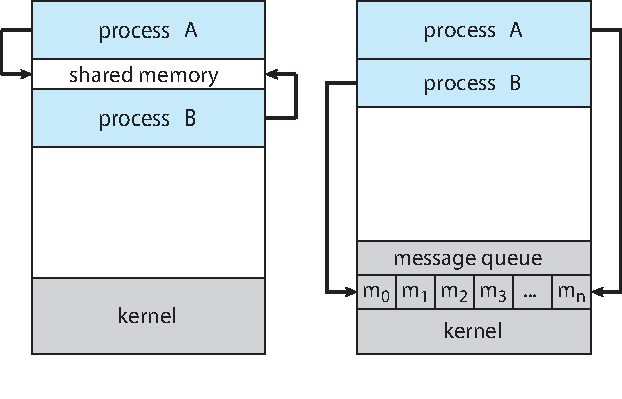
\includegraphics[height = 6cm]{figures/ipc_mechanisms.pdf}
    % \caption{} % \label{}
\end{figure}
Message passing is useful for exchanging small amounts of data, without
needing to avoid conflict. Shared memory can be faster than message
passing, as all accesses are treated as routine memory accesses, and no
assistance from the kernel is required, aside from establishing the
shared memory region.
\subsection{Shared Memory}
A common paradigm for shared memory is the \textbf{producer-consumer}
problem. A \textbf{producer} process \textit{produces} information that
is \textit{consumed} by the \textbf{consumer} process. For example, a
server might provide web content, which is read by a client web
browser.

A solution to this shared memory problem is to use a \textbf{buffer}
that is filled by the producer, and emptied by the consumer. In such a
system, the producer and consumer must be \textbf{synchronised} to
ensure the consumer does not try to consume data that has not yet been
produced.

Two types of buffers can be used:
\begin{itemize}
    \item \textbf{Unbounded buffer} --- the buffer has no fixed size;
          the producer can keep producing data, the consumer may need
          to wait if it is reading faster than the producer is writing
    \item \textbf{Bounded buffer} --- the buffer has a fixed size; the
          producer must wait if the buffer is full, and the consumer
          may need to wait if it is reading faster than the producer
\end{itemize}
In either case, at least one process is waiting for the other to either
write data, or to read data.

The shared buffer can be implemented using a circular array with two
pointers \mintinline{text}|in| and \mintinline{text}|out|.
\inputminted{c}{code/shared_memory.c} As the producer cannot write to
the buffer when the consumer points to the next location to be written,
the total number of items the buffer can hold is
\mintinline{text}|BUFFER_SIZE - 1|.
\subsection{Message Passing}
Message passing provides a mechanism to allow proesses to communicate
and to synchronise their actions without sharing the same address
space. It is particularly useful when communicating processes reside on
different computers that are connected by a network.

A message passing facility provides two operations:
\begin{itemize}
    \item \mintinline{text}|send(message)| --- send a message to another
          process
    \item \mintinline{text}|receive(message)| --- receive a message from
          another process
\end{itemize}
Messages sent by a process can be either \textbf{fixed} or
\textbf{variable} in size. If only fixed-size messages are sent, the
system-level implementation is more straightforward, however the task
of programming the application becomes more difficult. Conversely, if
variable-sized messages are sent, the system-level implementation is
more complex, but the task of programming the application becomes
easier.

If processes \(P\) and \(Q\) wish to communicate, they must
\begin{itemize}
    \item establish a \textbf{communication link} between them
    \item exchange messages via \textbf{send/receive} primitives
\end{itemize}
These links can be implemented in a variety of ways:
\begin{itemize}
    \item physically --- shared memory, hardware bus
    \item logically --- direct or indirect communication, synchronous
          or asynchronous communication, automatic or explicit
          buffering
\end{itemize}
\subsubsection{Naming}
Processes that want to communicate must be able to refer to each other.
This can be done either \textbf{directly} or \textbf{indirectly}.

Under direct communication, each process must explicity name the
recipient or sender of the communication:
\begin{itemize}
    \item \mintinline{text}|send(P, message)| --- send a message to
          process \(P\)
    \item \mintinline{text}|receive(Q, message)| --- receive a message
          from process \(Q\)
\end{itemize}
In this scheme, a link is established between each pair of processes
that wish to communicate. This allows for a \textbf{symmetric} or
\textbf{asymmetric} link to be established. The above example uses
symmetric addressing, but it is possible for the recipient to not
name the sender:
\begin{itemize}
    \item \mintinline{text}|send(P, message)| --- send a message to
          process \(P\)
    \item \mintinline{text}|receive(id, message)| --- receive a message
          from any process; the variable \(id\) is set to the name of
          the sender
\end{itemize}
The disadvantage of direct communication is the limited modularity of
the resulting system. If a process changes identifier, it may be
necessary to update all processes that communicate with it.

In contrast, \textbf{indirect communication} allows messages to be
passed to and from \textbf{mailboxes} or \textbf{ports}. Messages can
be placed into mailboxes and received by other processes that have
access to this shared mailbox. The \mintinline{text}|send()| and
\mintinline{text}|receive()| primitives are then extended to include
the name of the mailbox:
\begin{itemize}
    \item \mintinline{text}|send(A, message)| --- send a message to
          mailbox \(A\)
    \item \mintinline{text}|receive(A, message)| --- receive a message
          from mailbox \(A\)
\end{itemize}
In this method, we must decide how many processes can read from a
mailbox, or if they must take turns.
\subsubsection{Synchronisation}
Communication can be either \textbf{synchronous} or
\textbf{asynchronous}, also known as \textbf{blocking} and
\textbf{non-blocking} respectively. In relation to message passing,
this means:
\begin{itemize}
    \item \textbf{Blocking send}. The sending process must wait until
          the sent message is received by the receiving process
    \item \textbf{Non-blocking send}. The sending process can send a
          message and resume operation immediately
    \item \textbf{Blocking receive}. The receiving process must wait
          until a message is available
    \item \textbf{Non-blocking receive}. The receiving process can
          receive a valid message or null
\end{itemize}
If both send and receive are blocking, there is a \textbf{rendezvous}
between the sender and receiver.
\subsection{POSIX Shared Memory}
This section explores a mechanism for shared memory provided by the
POSIX API.\ POSIX shared memory is organised using
\textbf{memory-mapped} files that associate a region of shared memory
with a file. A process must first create a shared-memory object using
the \mintinline{text}|shm_open()| system call:
\inputminted{c}{code/posix_shared_memory_producer.c} The consuming
process can then read the contents of this shared memory using the code
below. \inputminted{c}{code/posix_shared_memory_consumer.c}
\subsubsection{Pipes}
Pipes allow two processes to communicate with each other through
message passing. The producer writes to the \textbf{write end} of the
pipe, and the consumer reads from the \textbf{read end} of the pipe. As
a result, pipes are \textbf{unidirectional}, and only allow one-way
communication. Below is an example of a pipe being used to communicate
between a parent and child process.

\inputminted{c}{code/pipe.c}
\section{Threads}
The process model described above implies that a process is a program
with a \textbf{single thread of execution}. However, most modern
operating systems allow processes to have multiple threads of
execution. Identifying opportunities for parallelism in a program is a
very important in multicore systems with multiple CPUs.
\subsection{Overview}
A \textbf{thread} is a basic unit of CPU utilisation, consisting of a
thread ID, a program counter, a register set, and a stack. It shares
with other threads belonging to the same process its code section, data
section, and other operating-system resources, such as open files and
signals. If a process has multiple threads of control, it can perform
more than one task at a time.
\begin{figure}[H]
    \centering
    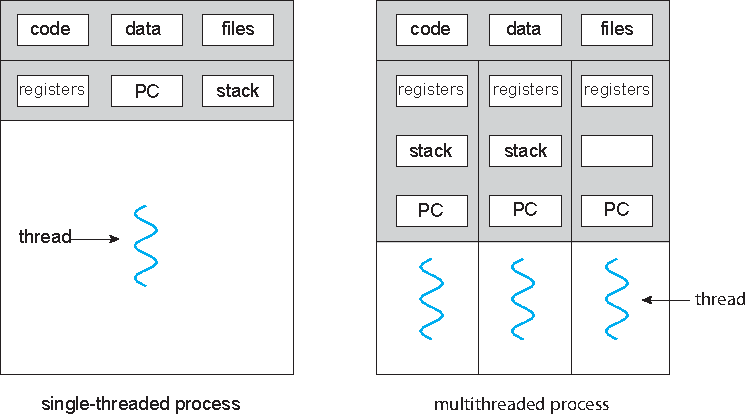
\includegraphics[height = 6cm]{figures/threads.pdf}
    % \caption{} % \label{}
\end{figure}
\subsubsection{Motivation}
Many modern applications are designed to leverage processing on
multicore systems to perform multiple tasks in parallel across multiple
computing cores. For example, a web server may have one thread to
listen for incoming requests, and another thread to process these
requests. Most operating system kernels are also multi-threaded.

As process creation is time consuming and resource intensive, it is
more efficient to use one process with multiple threads.
\subsubsection{Benefits}
There are several benefits to multi-threaded programming:
\begin{itemize}
    \item \textbf{Responsiveness} --- may allow continued execution if
          part of a process is blocked. This is especially important
          for user interfaces.
    \item \textbf{Resource sharing} --- threads share resources of the
          process to which they belong, including memory and files.
          This is easier than using shared memory or message passing.
    \item \textbf{Economy} --- creating and managing threads is
          generally faster than creating and managing processes. Context
          switching between threads incurs less overhead than between
          processes.
    \item \textbf{Scalability} --- multi-threaded programs can take
          advantage of multiprocessor architectures, as threads can be
          run in parallel on different processing cores.
\end{itemize}
\subsection{Multicore Programming}
Consider the following application with four threads. On a system with
a single computing core, concurrency is achieved by time slicing the
CPU between the threads executing only one thread at a time. On a
system with multiple cores, concurrency is achieved by running the
threads in parallel on different cores, because the system can assign a
separate thread to each core.
\begin{figure}[H]
    \centering
    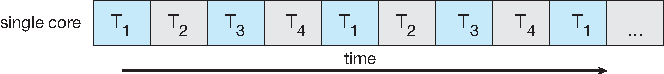
\includegraphics[width = 7cm]{figures/threads_single_core.pdf}
    % \caption{} % \label{}
\end{figure}
\begin{figure}[H]
    \centering
    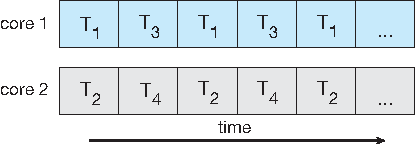
\includegraphics[width = 7cm]{figures/threads_multi_core.pdf}
    % \caption{} % \label{}
\end{figure}
Note the distinction between \textbf{parallelism} and \textbf{concurrency}.
\begin{itemize}
    \item A \textbf{concurrent} system supports more than one task by
          allowing all tasks to make process. On a single core system,
          the scheduler switches between tasks to achieve this.
    \item A \textbf{parallel} system can perform more than one task
          simultaneously.
\end{itemize}
Thus, a concurrent system does not imply it is also parallel.
There are two types of parallelism:
\begin{itemize}
    \item \textbf{Data parallelism} --- distributes subsets of the same
          data across multiple cores, performing the same operation on
          each core.
    \item \textbf{Task parallelism} --- distributes tasks (threads)
          across multiple computing cores, each of which performs a
          unique operation.
\end{itemize}
Note that these two types of parallelism are not mutually exclusive, and
an application may use a combination of both.
\subsubsection{Programming Challenges}
Multicore systems introduce several challenges for programmers to make
better use of multiple computing cores. Designers of oeprating systems
must write their own scheduling altorithms that use multiple cores to
allow parallel execution of threads. In general, there are five areas
that present challenges:
\begin{itemize}
    \item \textbf{Identifying tasks} --- identifying tasks that can be
          divided into separate, concurrent tasks. Ideally, these tasks
          are independent of one another, and can run on individual
          cores.
    \item \textbf{Balance} --- ensuring that all cores perform an equal
          amount of work. When one task contributes significantly less
          value than others, it may be necessary to use a separate
          execution core.
    \item \textbf{Data splitting} --- dividing data into subsets that
          can be operated on in parallel.
    \item \textbf{Data dependency} --- ensuring that tasks which access
          the same data are synchronised.
    \item \textbf{Testing and debugging} --- testing and debugging
          multi-threaded programs is more difficult than single-threaded
          programs.
\end{itemize}
\begin{tcolorboxlarge}[title={Amdahl's Law}, parbox=false]
    Amdahl's Law is a formula that identifies performance gains from
    adding additional cores, to an application that has both serial
    and parallel components. If \(S\) is the fraction of the application
    that must be performed serially on a system with \(N\) cores, then
    \begin{equation*}
        \text{speedup} = \frac{1}{S + \frac{1 - S}{N}}.
    \end{equation*}
\end{tcolorboxlarge}
\subsection{Multithreading Models}
Support for threads can be provided either at the user level, for
\textbf{user threads}, or at the kernel level, for \textbf{kernel
threads}. User threads are managed by user-level threads libraries such
as:
\begin{itemize}
    \item POSIX Pthreads
    \item Windows threads
    \item Java threads
\end{itemize}
Kernel threads are managed directly by the operating system, and this is
the case for most modern operating systems, such as Windows, Linux, and
macOS.
\begin{figure}[H]
    \centering
    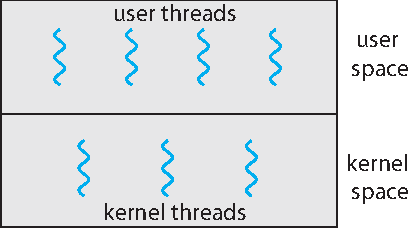
\includegraphics[width = 7cm]{figures/threads_user_kernel.pdf}
    % \caption{} % \label{}
\end{figure}
For the user space to utilise multiple cores, a relationship must be
established between user threads and kernel threads. The following
sections will explore various models that achieve this.
\subsubsection{Many-to-One Model}
The many-to-one model maps many user-level threads to a single kernel
thread. Thread managemen is done by the thread library in user space,
so it is efficient. However, an entire process will be blocked if a
thread makes a blocking system call. Additionally, because only one
thread can access the kernel at a time, multiple threads are unable to
run in parallel on multicore systems.
\begin{figure}[H]
    \centering
    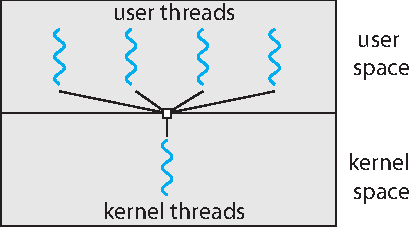
\includegraphics[width = 7cm]{figures/threads_many_to_one.pdf}
    % \caption{} % \label{}
\end{figure}
\subsubsection{One-to-One Model}
The one-to-one model maps each user thread to a kernel thread, and is
the most common approach. This allows multiple threads to run in
parallel on multicore systems. However, creating a user thread requires
creating a kernel thread, which is expensive and thus a large number of
kernel threads may affect performance.
\begin{figure}[H]
    \centering
    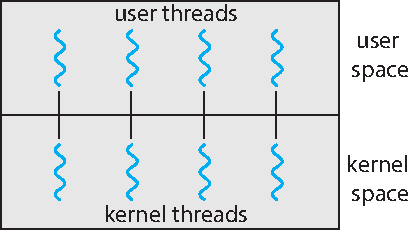
\includegraphics[width = 7cm]{figures/threads_one_to_one.pdf}
    % \caption{} % \label{}
\end{figure}
\subsubsection{Many-to-Many Model}
The many-to-many model multiplexes any number of user threads to an
equal or smaller number of kernel threads. This model allows the
operating system to create a sufficient number of kernel threads for a
particular application or machine. Although this model is the most
flexible, it is also the most difficult to implement.
\begin{figure}[H]
    \centering
    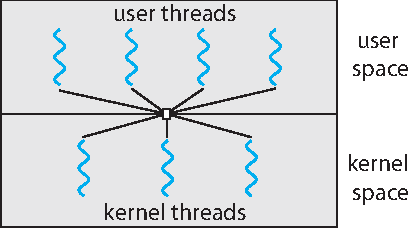
\includegraphics[width = 7cm]{figures/threads_many_to_many.pdf}
    % \caption{} % \label{}
\end{figure}
\subsubsection{Two-Level Model}
A two-level model is similar to the many-to-many model, but allows a
user thread to be bound to a kernel thread.
\begin{figure}[H]
    \centering
    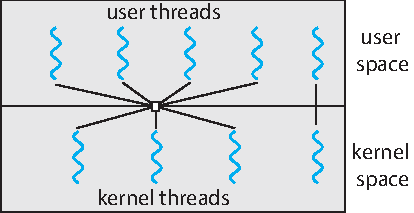
\includegraphics[width = 7cm]{figures/threads_two_level.pdf}
    % \caption{} % \label{}
\end{figure}
\subsection{Thread Libraries}
Thread libraries provide the programmer with an API for creating and
managing threads. There are two primary ways of implementing a thread:
\begin{itemize}
    \item User-level library, where support is limited to the user
          space.
    \item Kernel-level library, which is supported by the operating
          system.
\end{itemize}
Three thread libraries are in use today:
\begin{itemize}
    \item POSIX Pthreads --- a threads extension of the POSIX standard
          which may be provided as either a user-level or kernel-level
          library.
    \item Windows threads --- a kernel-level library that is part of
          the Windows API.
    \item Java threads --- a user-level library provided managed
          directly in Java programs.
\end{itemize}
There are two strategies for creating multiple threads:
\begin{itemize}
    \item \textbf{Asynchronous threading} --- the parent thread
          continues to execute concurrently and independently with the
          child thread it created. This is useful for tasks that
          require little data sharing between threads.
    \item \textbf{Synchronous threading} --- the parent thread waits
          until the child thread completes before continuing. This is
          useful for tasks that require significant data sharing
          between threads, where a parent thread may need to combine the
          results of multiple child threads.
\end{itemize}
\subsubsection{Pthreads}
Pthreads refers to the POSIX standard (IEEE 1003.1c) defining an API
for thread creation and synchronisation. This is a specification for
thread behaviour, not an implementation. Systems that implement the
Pthreads specification include UNIX-type operating systems such as
Linux and macOS.

The following program calculates the sum of the first \(n\) integers
using a multi-threaded program that follows the Pthreads API.
\inputminted{c}{code/pthreads_multithreading.c} In this program, the
\mintinline{c}|sum| variable is shared between the parent and child
threads. Each child thread begins control within the
\mintinline{c}|runner| function.

The parent thread waits for all child threads to complete by calling
the \mintinline{c}|pthread_join()| function.
\subsection{Implicit Threading}
To address the challenges of creating and managing threads, many
programming languages transfer these responsibilities to compilers and
run-time libraries. This is known as \textbf{implicit threading}. The
programmer must then identify tasks, rather than threads, that can be
executed in parallel. These tasks are usually defined as functions that
can be mapped to a separate thread, typically using the many-to-many
model. Three common approaches to implicit threading are discussed
below.
\subsubsection{Thread Pools}
A \textbf{thread pool} is a collection of worker threads that are
created at start-up and placed into a pool, where they wait for work.
When a task is to be performed, a thread is removed from the pool and
assigned to the task. When the task is complete, the thread returns to
the pool and waits for more work.

This approach has the following advantages:
\begin{itemize}
    \item Overhead of thread creation is avoided by servicing requests
          using an existing thread.
    \item The number of threads available can be bounded to the size of
          the pool.
    \item The separation of task submission from thread management
          allows for different strategies for scheduling tasks on
          threads. For example, a task can be scheduled to execute
          periodically.
\end{itemize}
Thread pools are supported by the Windows API.
\subsubsection{OpenMP}
OpenMP is a set of compiler directives and an API for C, C++, and
Fortran that provides support for parallel programming in shared-memory
environments. OpenMP identifies \textbf{parallel regions} as blocks of
code that may run in parallel. These regions are defined using
\mintinline{c}|#pragma| directives as shown below.

\inputminted{c}{code/openmp.c}

In this code, the \mintinline{c}|#pragma omp parallel| directive
creates as many threads as cores in the system, and all threads execute
the code within the parallel region. To parallelise loops, the
\mintinline{c}|#pragma omp parallel for| directive can be used to
distribute the iterations of a for loop across threads.

OpenMP also allows developers to specify the number of threads
manually, and identify whether data should be shared or private to each
thread. OpenMP is available on several open-source and commercial
compilers for Linux, Windows, and macOS systems.
\subsubsection{Grand Central Dispatch}
Grand Central Dispatch (GCD) is a technology developed by Apple for
macOS and iOS. It is a combination of a run-time library, API, and
language extension that allows developers to identify tasks that can be
executed in parallel. GCD manages most of the details of threading.

GCD schedules tasks for run-time execution by placing them in a
\textbf{dispatch queue}. When a task is ready to execute, it is removed
from this queue and assigned to an available thread from a thread pool.
There are two types of dispatch queues:
\begin{itemize}
    \item \textbf{Serial queues} --- tasks are executed in FIFO order,
          and a task must be completed before the next task is executed.
          This queue is called the \textbf{main queue} of a process.
    \item \textbf{Concurrent queues} --- tasks are also executed in
          FIFO order, but multiple tasks may be removed at a time,
          allowing them to be executed in parallel.
          These tasks are prioritised into three system wide queues.
\end{itemize}
In C, GCD defines a language extension called a \textbf{block} that is a
self-contained unit of work specified by a caret (\mintinline{c}|^|):
\begin{minted}{c}
^{ /* code */ }
\end{minted}
\subsection{Threading Issues}
This section discusses issues that arise when designing multi-threaded
programs.
\subsubsection{\mintinline{c}|fork()| and \mintinline{c}|exec()| System Calls}
The semantics of the \mintinline{c}|fork()| system call in a
multi-threaded program may not be well defined. If a thread calls
\mintinline{c}|fork()|, does the new process duplicate all threads, or
is the new process single-threaded? In some UNIX systems, two versions
of the \mintinline{c}|fork()| system call are defined to address this
ambiguity.

In the case of a thread calling \mintinline{c}|exec()|, the new program
specified will usually replace the entire process, including all
threads.
\subsubsection{Signal Handling}
Signals are used in UNIX systems to notify a process that a particular
event has occurred. For example, illegal memory access or division by
0. Signals may be received both synchronously and asynchronously, and
follow the same pattern:
\begin{enumerate}
    \item A signal is generated by a particular event.
    \item The signal is delivered to a process.
    \item The signal is handled by either a default or user-defined
          signal handler.
\end{enumerate}
Every signal has a default handler that the kernel runs when handling
that signal. This may be overriden by a user-defined signal handler.
Some signals may be ignored, whereas some signals terminate the program.

For single-threaded applications, signals are delivered to the process.
However, it is not clear where a signal should be delivered in a
multi-threaded application. One of the following options exist:
\begin{itemize}
    \item Deliver the signal to the thread to which the signal applies.
    \item Deliver the signal to every thread in the process.
    \item Deliver the signal to certain threads in the process.
    \item Assign a specific thread to receive all signals for the
          process.
\end{itemize}
\subsubsection{Thread Cancellation}
Thread cancellation terminates a thread before it has completed. For
example, if multiple threads are concurrently searching a large data
structure, and one thread finds the result, the other threads may be
cancelled.

The thread to be cancelled is called the \textbf{target thread}, and
there are two ways to cancel this thread:
\begin{itemize}
    \item \textbf{Asynchronous cancellation} --- terminates the target
          thread immediately.
    \item \textbf{Deferred cancellation} --- allows the target thread
          to periodically check if it should be cancelled.
\end{itemize}
This poses a difficulty when resources are shared between threads.
For example, if a thread is cancelled while it is modifying data shared
with other threads, it is not possible to reclaim all resources used by
the target thread, as other threads may be using them.

In Pthreads, the \mintinline{c}|pthread_cancel()| function indicates a
request to cancel the target thread, which may be deferred or
asynchronous. Program cancellation occurs when the thread reaches its
\textbf{cancellation point}. A cancellation point can be specified
using \mintinline{c}|pthread_testcancel()|, which checks if a
cancellation request has been made.

A \textbf{cleanup handler} may be invoked to release any resources
before the thread is terminated.
\subsubsection{Thread-Local Storage}
Thread-local storage allows threads to have a separate copy of shared
data in a process. This is useful when the thread the developer has no
control over the thread creation process.

This data has a similar visibility to static variables, but it is
unique to each thread.
\subsubsection{Scheduler Activations}
Systems implementing the many-to-many and two-level threading models
require communication between the kernel and thread library to allow
the number of kernel threads allocated to the program to be adjusted
dynamically. This is done using an intermediate data structure between
user and kernel threads, known as a \textbf{lightweight process} (LWP).
\begin{figure}[H]
    \centering
    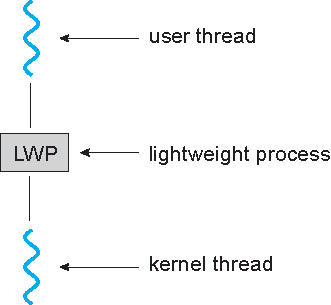
\includegraphics[height = 4cm]{figures/lwp.pdf}
    % \caption{} % \label{}
\end{figure}
To the user-thread library, the LWP appears as a virtual processor on
which the process can schedule a user thread to run. Each LWP is
attached to a kernel thread, and it is the kernel thread that is
scheduled by the operating system.

One scheme for communication is known as \textbf{scheduler activation}.
In this scheme, the kernel provids an application with a set of virtual
processors (LWPs). The kernel informs an application about events using
an \textbf{upcall} that are handled by the thread library in an
\textbf{upcall handler}.
\section{Synchronisation}
A cooperating process is a process that can affect other processes in a
system. These processes allow concurrent access of data which may
result in data inconsistency. This section explores the various
mechanisms that can be used to ensure consistency.
\subsection{Background}
Processes executing concurrently or in parallel may be interrupted at
any point in their execution, even if that process has partially
completed an operation.

Consider an updated producer-consumer shared memory implementation,
where the producer and consumer access a shared variable
\mintinline{c}|count| to allow the entire buffer to be utilised. This
variable counts the number of items not yet consumed by the consumer.
\inputminted{c}{code/producer_consumer_synchronisation.c} Assuming
\mintinline{c}|count = 5| initially, and the increment and decrement
operations are implemented in Assembly like so:
\begin{minted}{c}
register1 = count;
register1 = register1 + 1;
count = register1;

register2 = count;
register2 = register2 - 1;
count = register2;
\end{minted}
then if during the concurrent execution of this program, the CPU
executes these instructions in the following manner:
\begin{minted}{c}
register1 = count;         // producer, register1 = 5
register1 = register1 + 1; // producer, register1 = 6
// interrupt
register2 = count;         // consumer, register2 = 5
register2 = register2 - 1; // consumer, register2 = 4
// interrupt
count = register1;         // producer, count = 6
// interrupt
count = register2;         // consumer, count = 4
\end{minted}
then, the resulting value of \mintinline{c}|count| will incorrectly be
4, rather than 5.

The situation where multiple processes manipulate the value of the same
variable concurrently, where the order in which access to the variable
occurs is important, is known as a \textbf{race condition}.

To guard against the race condition encountered above, processes need
to be synchronised.
\subsection{The Critical-Section Problem}
Consider a system consisting of \(n\) processes \(\left\{ P_0,\: P_1,\:
\dots,\: P_{n-1} \right\}\), each of which has a segment of code,
called a \textbf{critical section}, in which the process may access and
update data shared with at least one other process. In this system, no
two processes may be simultaneously inside their critical sections.

The solution to this problem splits the program into the following
sections:
\begin{itemize}
    \item entry section
    \item critical section
    \item exit section
    \item remainder section
\end{itemize}
Each process requests permission to enter its critical section in the
entry section. Once it has finished executing its critical section, the
process may be followed by an exit section, to indicate that it has
finished. The remainder section consists of any code that is not
critical.

This solution must also satisfy the following three requirements:
\begin{itemize}
    \item \textbf{Mutual exclusion} --- if process \(P_i\) is executing
          in its critical section, then no other processes can be
          executing in their critical sections.
    \item \textbf{Progress} --- if no process is currently executing in
          its critical section, then only those processes not in their
          remainder section may participate in the decision of which
          process will enter its critical section next. This decision must
          be made in a finite amount of time.
    \item \textbf{Bounded waiting} --- there exists a bound on the
          number of times that a process requests to enter its critical
          section before that request is granted. This prevents a
          process from waiting forever to enter its critical section.
\end{itemize}
Here we assume that each process executes at a nonzero speed but there
is no assumption concerning the relative speed of the \(n\) processes.

There are two approaches to handle critical sections depending on the
kernel:
\begin{itemize}
    \item \textbf{Preemptive kernel} --- the kernel may pre-empt
          (interrupt) a process while it is executing in kernel mode.
    \item \textbf{Non-preemptive kernel} --- the kernel does not
          pre-empt (interrupt) a process while it is executing in
          kernel mode.
\end{itemize}
While the non-preemptive kernel is free of race conditions, it may be
more repsonsive as there is no risk that a process will run forever.
\subsection{Peterson's Solution}
Peterson's solution is a two process solution to the critical section
problem which uses two variables to control access to the critical
section. An implementation of Peterson's solution is shown below.

\inputminted{c}{code/petersons_solution.c}

A problem with this solution is that the operating system is free to
reorder instructions to optimise runtime, resulting in both threads
entering their critical sections at the same time.
\subsection{Hardware Support for Synchronisation}
The above solution is a \textit{software-based} solution as it does not
rely on any special support from the operating system or hardware, to
ensure mutual exclusion.

As will be discussed in the next section, locks are a common mechanism
for ensuring mutual exclusion. Locks can be used to prevent a process
from entering its critical section, if another process is already in
its critical section.
\subsubsection{Atomic}
An \textbf{atomic operation} is an indivisible operation that cannot be
interrupted by the operating system.

\textbf{Atomic variables} provide atomic operations on basic data types
such as integers, and can be modified by multiple threads without race
conditions.
\subsection{Mutex Locks}
A \textbf{mutex lock} (mutual exclusion lock) is a lock that can be
used to ensure mutual exclusion. A mutex lock protects critical
sections and thus prevents race conditions. A mutex lock has two
operations:
\begin{itemize}
    \item \mintinline{c}|acquire()| --- if the lock has been released,
          acquire it, otherwise wait until it is.
    \item \mintinline{c}|release()| --- release the lock.
\end{itemize}
A thread cannot enter its critical section until it has acquired the
mutex lock and must release the mutex lock when it exits its critical
section. These functions can be implemented as follows:
\begin{minted}{c}
acquire()
{
    while (!available)
        ; // busy wait

    available = false;
}

release()
{
    available = true;
}

do
{
    acquire();
    // critical section
    release();
    // remainder section
} while (true);
\end{minted}
The calls to \mintinline{c}|acquire()| and \mintinline{c}|release()|
must be \textbf{atomic}.

A problem with this implementation is that it requires \textbf{busy
waiting} where a thread waits for a condition to met without yielding
control to the operating system. This is wasteful as it consumes CPU
cycles that could be used by other threads.

This particular scenario is known as a \textbf{spinlock}, as lock
contention is low, and the thread is likely to acquire the lock after a
short duration. Here waiting is more efficient than performing a
context switch to another thread.
\subsection{Semaphores}
Semaphores are similar to mutex locks, but allow multiple threads to
access a shared resource simultaneously. Semaphores can be accessed by
two atomic operations:
\begin{itemize}
    \item \mintinline{c}|wait()| --- if the value of the semaphore is
          nonzero, decrement it and continue, otherwise, wait until it
          is.
    \item \mintinline{c}|signal()| --- increment the value of the
          semaphore.
\end{itemize}
The number a semaphore is initialised to is the number of threads that
are allowed to access the shared resource simultaneously. If this number
is equal to 1, the semaphore is called a \textbf{binary semaphore}, and
is equivalent to a mutex lock. When a semaphore is initialised to a value
greater than 1, it is called a \textbf{counting semaphore}. Semaphores
can be implemented as follows:
\begin{minted}{c}
wait(S)
{
    while (S <= 0)
        ; // busy wait

    S--;
}

signal(S)
{
    S++;
}

do
{
    wait(S);
    // critical section
    signal(S);
    // remainder section
} while (true);
\end{minted}
where both \mintinline{c}|wait()| and \mintinline{c}|signal()| must be
atomic.
\subsubsection{Precedence}
If a process must be executed before another process, a semaphore can
be used to enforce this precedence. Given processes \(P_1\) and \(P_2\)
with statements \(S_1\) and \(S_2\) respectively, if \(P_1\) must be
executed before \(P_2\), then the following code can be used:
\begin{minted}{c}
// P1
S1;
signal(S);

// P2
wait(S);
S2;
\end{minted}
where \(S\) is a binary semaphore initialised to 0. This code requires
\(P_1\) to signal \(S\) before \(P_2\) can execute.
\subsubsection{Non-Busy Waiting}
Both mutex locks and the above implementation of the semaphore require
threads to busy wait. This can be avoided by \textbf{suspending}
threads that need to wait for a semaphore. This is done by maintaining
a queue of suspended threads, where each suspended thread transfers
control to the CPU scheduler. When a thread has released a semaphore,
it must wake up a thread from the queue. An implementation of this is
shown below:
\begin{minted}{c}
typedef struct
{
    int value;
    struct process *list;
} semaphore;

void wait(semaphore *S)
{
    S->value--;
    if (S->value < 0)
    {
        // add this process to S->list;
        sleep();
    }
}

void signal(semaphore *S)
{
    S->value++;
    if (S->value <= 0)
    {
        // remove a process from S->list;
        wakeup();
    }
}

do
{
    wait(S);
    // critical section
    signal(S);
    // remainder section
} while (true);
\end{minted}
In this implementation, semaphore values may be negative to allow the
number of waiting threads to be tracked as the absolute value of the
semaphore value.
\subsubsection{Deadlock and Starvation}
A \textbf{deadlock} occurs when two or more threads are waiting for an
event that can only be caused by one of the waiting threads. In the
following example, both thread 0 and 1 are waiting for the other thread
to release the semaphore, resulting in a deadlock.
\begin{minted}{c}
// thread 0
wait(S0);
wait(S1);
signal(S0);
signal(S1);

// thread 1
wait(S1);
wait(S0);
signal(S1);
signal(S0);
\end{minted}
A \textbf{starvation} occurs when a thread is perpetually denied access
to a resource. This can occur when a thread has a lower priority than
other threads, and thus is never scheduled.
\subsubsection{Semaphore Problems}
Semaphores may be misused in the following ways:
\begin{itemize}
    \item If a \mintinline{c}|signal()| operation is executed before a
          \mintinline{c}|wait()| operation, the mutual-exclusion
          requirement will be violated.
    \item If a \mintinline{c}|wait()| operation is executed twice
          without an intervening \mintinline{c}|signal()| operation,
          the thread will permanently block on the second call to
          \mintinline{c}|wait()| as the semaphore value will be
          unavailable.
    \item If either \mintinline{c}|wait()| or \mintinline{c}|signal()|
          is omitted, mutual exclusion may be violated, or the thread
          will block indefinitely.
\end{itemize}
\subsection{Monitors}
Monitors are a high-level abstraction that provide a convenient and
effective mechanism for process synchronisation. This reduces the risk
of programmer error when using semaphores.

A monitor is an \textbf{abstract data type} (ADT) that encapsulates
data with a set of methods that operate on that data. A monitor is
defined as follows:
\begin{minted}{c}
monitor monitor-name
{
    // shared variable declarations
    // procedures that operate on the shared variables
    procedure P1(...) { ... }
    ...
    procedure Pn(...) { ... }

    // initialisation code
    initialisation(...) { ... }
}
\end{minted}
where each operation within this monitor is mutually exclusive. All
internal variables must only be accessed by the procedures within the
monitor, and local variables must be private to each procedure. The
monitor maintains a queue of threads waiting to enter the monitor, and
only one thread may be executing within the monitor at any time.

This is not sufficient to model certain synchronisation problems, and
therefore, monitors also provide the \textbf{condition construct}.
\begin{minted}{c}
condition x, y;
\end{minted}
A condition variable has two operations:
\begin{itemize}
    \item \mintinline{c}|wait()| --- a thread that invokes an operation
          is suspended until another thread invokes
          \mintinline{c}|signal()|.
    \item \mintinline{c}|signal()| --- resumes a process (if any) which
          called \mintinline{c}|wait()|. This function may be called
          multiple times, and has no effect if no threads are suspended.
\end{itemize}
\subsection{Classical Problems of Synchronisation}
This section explores three classical problems of synchronisation, and
provides solutions using the concepts discussed above.
\subsubsection{The Bounded-Buffer Problem}
In this problem, processes produce and consume data from a shared
buffer of size \(n\). The solution to this problem requires the
following shared data:
\begin{minted}{c}
#define BUFFER_SIZE n
semaphore mutex = 1; // controls access to critical section
semaphore empty = N; // counts empty buffer slots
semaphore full = 0;  // counts full buffer slots
\end{minted}
The producer and consumer can be implemented as follows:
\begin{minted}{c}
// producer
while (true)
{
    /* produce an item */
    wait(empty);
    wait(mutex);
    /* add item to buffer */
    signal(mutex);
    signal(full);
}

// consumer
while (true)
{
    wait(full);
    wait(mutex);
    /* remove item from buffer */
    signal(mutex);
    signal(empty);
    /* consume the item */
}
\end{minted}
\subsubsection{The Readers-Writers Problem}
In this problem, a data set is shared among a number of concurrent
processes, where some processes only read the data, and others can both
read and write the data. In the following solution, the data set is
protected by two semaphores:
\begin{minted}{c}
semaphore mutex = 1;    // control access to read_count variable
semaphore rw_mutex = 1; // controls access to data
int read_count = 0;     // number of readers accessing data
\end{minted}
The reader and writer processes can be implemented as follows:
\begin{minted}{c}
// reader
while (true)
{
    wait(mutex); // ensure exclusive access to read_count
    read_count++;
    if (read_count == 1)
        wait(rw_mutex);  /* first reader locks data */
    signal(mutex);
    /* read data */
    wait(mutex); // ensure exclusive access to read_count
    read_count--;
    if (read_count == 0)
        signal(rw_mutex); /* last reader unlocks data */
    signal(mutex);
}

// writer
while (true)
{
    wait(rw_mutex); // ensure exclusive access to data
    /* write data */
    signal(rw_mutex);
}
\end{minted}
\subsubsection{The Dining-Philosophers Problem}
In this problem, \(n\) philosophers sit around a table with a bowl of
rice in the centre. These philosophers spend their lives thinking and
eating. Each philosopher has a plate of food in front of them, with
chopsticks between each plate.

This problem has the following constraints:
\begin{itemize}
    \item When a philosopher is hungry, they will try to pick up the
          two chopsticks adjacent to their plate, one at a time. They
          cannot take a chopstick that is held by a neighbouring
          philosopher.
    \item When a philosopher has two chopsticks, they may eat for a
          finite amount of time.
    \item When a philosopher is finished eating, they must put down
          both chopsticks and think.
    \item When a philosopher is thinking, they do not need any
          chopsticks.
\end{itemize}
The first solution to this problem uses semaphores. Consider the shared
data:
\begin{minted}{c}
semaphore chopstick[n];
\end{minted}
where all elements of this array are initialised to 1. The philosopher
processes can be implemented as follows:
\begin{minted}{c}
// philosopher i
while (true)
{
    wait(chopstick[i]);
    wait(chopstick[(i + 1) % n]);
    /* eat */
    signal(chopstick[i]);
    signal(chopstick[(i + 1) % n]);
    /* think */
}
\end{minted}
This solution is correct, but may result in \textbf{starvation} as a
philosopher may never be able to acquire both chopsticks if other
philosophers are constantly eating. Additionally, if all philosophers
are hungry at the same time, they may all acquire one chopstick and
wait forever for the other, resulting in a \textbf{deadlock}.

To solve the problem of deadlock, a monitor can be used.
\begin{minted}{c}
monitor DiningPhilosophers
{
    enum { THINKING, HUNGRY, EATING } state[n];
    condition self[n];

    void pickup(int i)
    {
        state[i] = HUNGRY;      // ith philosopher is hungry
        test(i);                // try to eat
        if (state[i] != EATING) // if unable to eat
            self[i].wait();     // wait to be signalled
    }

    void putdown(int i)
    {
        state[i] = THINKING;   // ith philosopher is thinking
        test((i + n - 1) % n); // allow left neighbour to eat if hungry
        test((i + 1) % n);     // allow right neighbour to eat if hungry
    }

    void test(int i)
    {
        // if neither neighbour is eating
        // and ith philosopher is hungry
        if ((state[(i + n - 1) % n] != EATING) &&
            (state[i] == HUNGRY) &&
            (state[(i + 1) % n] != EATING))
        {
            state[i] = EATING;
            self[i].signal();  // signal ith philosopher to eat
        }
    }

    initialisation()
    {
        for (int i = 0; i < n; i++)
            state[i] = THINKING;
    }
}
\end{minted}
This solution ensures that a philosopher only picks up a chopstick if
both of their neighbours are not eating. This prevents deadlock as
there will always be at least one philosopher that can eat.
\section{Safety Critical Systems}
Safety critical systems are systems whose failure may result in one of
the following outcomes:
\begin{itemize}
    \item illness, serious injury, or death
    \item damage to or loss of equipment or property
    \item damage to the environment
\end{itemize}
The increase of software in safety critical systems necessitates the
proper design and implementation of these systems.
\subsection{Safety Critical Software}
Software is not inherently safe or unsafe. However the use of software
in a safety critical system may contribute to an unsafe situation. Such
software is considered safety critical.

Low risk systems are safety related, whereas high risk systems are
safety critical.
\subsection{Dependability}
Dependability is the most important property of a system critical
system. It reflects the user's confidence in a system. The costs of
system failure are often very high, and so dependability covers a range
of attributes such as:
\begin{itemize}
    \item \textbf{Reliability} --- The ability to deliver services as
          specified.
    \item \textbf{Availability} --- The ability to deliver services
          when required.
    \item \textbf{Safety} --- The ability to operate without
          catastrophic failure.
    \item \textbf{Security} --- The ability to protect itself against
          accidental or deliberate intrusion.
\end{itemize}
Both reliability and availability are measured as a probability of
failure over a given time period.
\subsection{Achieving Safety}
\begin{itemize}
    \item \textbf{Hazard avoidance} --- The system should be designed
          to avoid hazards.
    \item \textbf{Hazard detection and removal} --- The system
          should be designed to detect hazards and remove them
          before they cause accidents.
    \item \textbf{Damage limitation} --- The system should be designed
          to limit the damage caused by hazards.
\end{itemize}
In complex systems, accidents typically occur as a result of multiple
failures. As such, designing a system to be completely safe is
difficult.\ \textbf{Dependability costs} increase exponentially as
increasing levels of dependability are required, and therefore a
comprimise must be made between design cost and dependability.
\subsection{Risk Analysis}
Failures in safety critical systems can be caused by:
\begin{itemize}
    \item \textbf{Hardware failure} --- Manufacturing, end-of-life,
          or design error.
    \item \textbf{Software failure} --- Specification, design,
          or implementation errors.
    \item \textbf{Operational failure} --- Human or socio-technical
          errors.
\end{itemize}
\subsubsection{Hazard and Risk}
\begin{itemize}
    \item A \textbf{hazard} is a situation that has the potential to
          cause harm.
    \item \textbf{Risk} enacapsulates the probability that a hazard
          will lead to an accident, and the severity of the consequences
          of that accident. Risk is a product of the probability of
          accident and the severity of the consequences.
\end{itemize}
Risk analysis involves identifying hazards and limiting the risks
associated with them.
\subsubsection{Faults and Failures}
A \textbf{fault} is an event that may lead to a failure, whereas a
\textbf{failure} is the inability of a system or component to perform
its required function within specified limits.

Failures may be the result of one or more faults, and there are several
ways to trace a failure back to its cause:
\begin{itemize}
    \item \textbf{Failure mode and effects analysis} (FMEA) --- A
          systematic way of identifying the possible faults that may
          lead to a failure, and the consequences of that failure.
    \item \textbf{Failure tree analysis} (FTA) --- A graphical technique
          that can be used to analyse the combination of faults that may
          lead to a failure.
\end{itemize}
\subsection{Safety Standards}
Many standards have been developed to ensure the safety of software in
particular domains. One standard is the \textbf{International
Electrotechnical Commission} (IEC) 61508 standard, which is a generic
standard for functional safety. This standard has the following views
on risk:
\begin{itemize}
    \item Zero risk can never be reached, but the risk can be reduced
          to an acceptable level.
    \item Non-tolerable risks must be reduced as lot as reasonably
          possible.
    \item Optimal cost effective safety is achieved when addressed in
          the entire safety lifecycle.
\end{itemize}
IEC 61508 defines three successive tiers of safety assessments:
\begin{itemize}
    \item Safety Instrumented Systems (SIS) --- The entire system that
          is composed of Safety Instrumented Functions (SIF).
    \item Safety Instrumented Functions (SIF) --- A function
          implemented by the SIS that is intended to achieve or
          maintain a safe state for the process.
    \item Safety Integrity Level (SIL) --- A measure of the safety
          integrity requirements of a particular SIF. SIL 1 is low risk
          and therefore allows for a higher probability of failure, and
          SIL 4 is high risk and therefore requires a Lower probability
          of failure.
\end{itemize}
\subsection{Real-Time Operating Systems}
Real-time operating systems (RTOS) are operating systems that are
designed to meet the requirements of real-time applications. The
following considerations must be made when designing an RTOS:
\begin{itemize}
    \item \textbf{Tasking}
          \begin{itemize}
              \item Tasks terminating or deleting
              \item Overflows within a kernel's storage area for task
                    control blocks
              \item Tasks exceeding stack size limits
          \end{itemize}
    \item \textbf{Scheduling}
          \begin{itemize}
              \item Deadlocks
              \item Resource starvation
              \item Unbounded execution times
          \end{itemize}
    \item \textbf{Memory and I/O Access}
          \begin{itemize}
              \item Inappropriate pointer usage
              \item Data erasure
              \item Unauthorised access
          \end{itemize}
    \item \textbf{Queueing}
          \begin{itemize}
              \item Overflows
          \end{itemize}
    \item \textbf{Interrupt and Error Handling}
          \begin{itemize}
              \item Lack of error handling
              \item Lack of interrupt handling
              \item Improper protection of superisor tasks
          \end{itemize}
\end{itemize}
\subsection{DO-178B Standard}
The DO-178B standard is a software standard for airborne systems. It
consists of five main processes:
\begin{itemize}
    \item Software planning
    \item Software development
    \item Software verification
    \item Software configuration management
    \item Software quality assurance
\end{itemize}
\subsubsection{Software Planning Process}
The software planning process determins what needs to be done to
produce safe and requirements-based software. It's expected outputs
are:
\begin{itemize}
    \item A plan for software aspects of certification
    \item A plan for software development
    \item A plan for software verification
    \item A plan for software configuration management
    \item A plan for software quality assurance
\end{itemize}
\subsubsection{Software Development Process}
The software development process is broken into four sub-processes:
\begin{itemize}
    \item \textbf{Software requirements} --- High-level requirements in
          relation to functionality, performance, and safety.
    \item \textbf{Software design} --- Low-level requirements used
          to implement source code.
    \item \textbf{Software coding} --- Production of source code from
          the design process.
    \item \textbf{Software integration} --- Integration of software
          into a real-time environment.
\end{itemize}
This process is iterative, and the expected outputs are:
\begin{itemize}
    \item Software requirements data
    \item Software design description
    \item Source code
    \item Executable object code
\end{itemize}
\subsubsection{Software Verification Process}
Software verification consists of:
\begin{itemize}
    \item verification of software requirements
    \item validation of software design
\end{itemize}
these can be achieved through reviews, analysis, and testing.
This process outputs:
\begin{itemize}
    \item Software verification cases and procedures
    \item Software verification results
\end{itemize}
\subsubsection{Software Configuration Management Process}
The software configuration management process is used to establish
secure and effective configuration control for all artifacts. The
following activities may be conducted:
\begin{itemize}
    \item Identification of configuration items
    \item Change control
    \item Baseline establishment
    \item Software archival
\end{itemize}
This process outputs:
\begin{itemize}
    \item Software configuration index
    \item Software lifecycle environment configuration index
\end{itemize}
\subsubsection{Software Quality Assurance Process}
The software quality assurance process provides assurance that the
software life cycle process will yield quality software. Each process
is analysed to demonstrate that processes produce expected outputs.
Changes to originally proposed plans are reported, evaluated, and
resolved to ensure process integrity.
\subsection{Programming Standards}
While many languages are used in safety critical systems, certain
languages may be preferred for various purposes. Many C standards also
subset the language to remove features that are considered unsafe.
\subsubsection{MISRA C}
MISRA C is a set of guidelines on a subset of the C language in
critical systems. MISRA C has three levels of compliance:
\begin{itemize}
    \item \textbf{Mandatory} --- These rules must be followed without
          exception.
    \item \textbf{Required} --- These rules must be followed but may
          be violated in certain situations. These violations must also
          be documented.
    \item \textbf{Advisory} --- These rules should be followed but are
          not mandatory.
\end{itemize}
MISRA C is used for error prevention, rather than error detection,
and violation of a guideline does not necessarily mean that a program
is incorrect.
\section{Distributed Systems}
A distributed system is a collection of independent processors that do
not share memory or a clock. Each node in the system has its own local
memory, and communicates with other nodes through various networks.

A distributed system is a collection of loosely coupled nodes,
interconnected by a communication network. The processes in a
distributed system are called nodes, sites, machines, or hosts.

Nodes can exist in a \textbf{client-server}, \textbf{peer-to-peer}, or
\textbf{hybrid} configuration. In a client-server architecture,
\begin{itemize}
    \item \textbf{Site} refers to the physical location of a node
    \item \textbf{Servers} provide resources which \textbf{clients}
          want to use
\end{itemize}
\subsection{Advantages of Distributed Systems}
\begin{itemize}
    \item \textbf{Resource sharing} --- provides mechanisms for:
          \begin{itemize}
              \item sharing files at remote sites
              \item processing information in a distributed database
              \item printing files at remote sites
              \item using remote specialised hardware such as
                    supercomputers or graphical processing units
          \end{itemize}
    \item \textbf{Computation speedup} --- computation that can be
          partitioned into subcomputations can be distributed among several
          nodes. If a particular site is overloaded with requests, some
          requests can be moved or rerouted to other lightly loaded sites.
          This is known as \textbf{load balancing} or \textbf{job migration}.
    \item \textbf{Reliability} --- the failure of a node does not
          necessarily cause the failure of the entire system. The
          failure of a node must be detected by the system and
          appropriate actions must be taken to recover from the failure.
          This may include transferring the function of the failed node
          to another node.
    \item \textbf{Communication} --- high-level functions can be
          expanded to allow communication between processes on different
          machines.
\end{itemize}
\subsection{Network Structure}
Networks are used to connect nodes in a distributed system. There are
two types of network:
\begin{itemize}
    \item \textbf{Local-area network} (LAN) --- a network that covers
          a small geographical area, such as a single building or a
          cluster of buildings.
    \item \textbf{Wide-area network} (WAN) --- a network that covers
          a large geographical area, such as a country or the world.
\end{itemize}
These differences imply variations in the speed and reliability of the
communications networks, and these are reflected in the design of
distributed systems.
\subsubsection{Local-Area Networks}
Local-area networks are typically found in homes and offices, where it
is more economical to have a number of computers with their own
self-contained applications, than to have a single large system. To
allow some form of data sharing between these computers, a LAN is used.
Below are some characteristics of LANs:
\begin{itemize}
    \item LANs can take multiple forms, such as a bus, ring, or star
          topology.
    \item LANs provide communication speeds from \qty{1}{Mb.s^{-1}} to
          \qty{40}{Gb.s^{-1}} when using Ethernet over twisted pair
          copper or optical fibres.
    \item LANs consist of multiple different computers (including,
          workstations, servers, laptops, mobile devices), peripherals
          (such as printers, scanners, storage arrays), and specialised
          network communication processors like routers that provide
          access to other networks.
    \item Ethernet is the most common LAN technology, and is defined by
          the IEEE 802.3 standard.
    \item WiFi is increasingly used for networking and is defined by
          the IEEE 802.11 standard which is constantly evolving.
\end{itemize}
\begin{figure}[H]
    \centering
    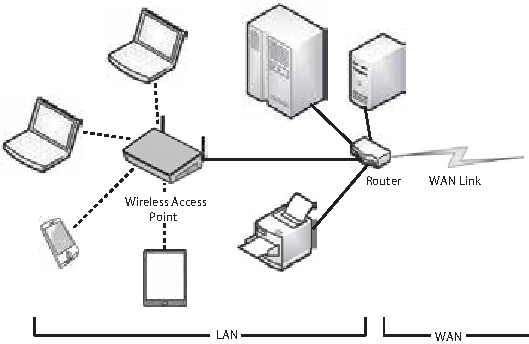
\includegraphics[height = 5cm]{figures/LAN.pdf}
    % \caption{} % \label{}
\end{figure}
\subsubsection{Wide-Area Networks}
Wide-area networks are typically used for communication over large
areas, such as between cities or countries. Communication links are
controlled by routers that forward messages between sites.

Hosts are generally on LANs, which are connected to the Internet
through routers. WANs are also slower than LANs due to the distances
they cover.
\begin{figure}[H]
    \centering
    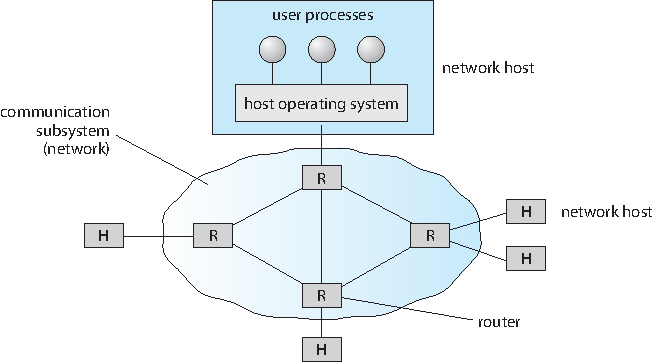
\includegraphics[height = 5cm]{figures/WAN.pdf}
    % \caption{} % \label{}
\end{figure}
\subsection{Network and Distributed Operating Systems}
There are two main categories of network-oriented operating systems.
\textbf{Network operating systems} are simpler to implement but
generally more difficult for users to access and use.
\textbf{Distributed operating systems} provide more features.
\subsubsection{Network Operating Systems}
Network operating systems provide environments for users to access
remote resources, and this is done explicitly by:
\begin{itemize}
    \item \textbf{Remote Login} --- Logging into machines remotely
          through ssh or telnet.
    \item \textbf{Remote File Transfer} --- Transferring data between
          local and remote machines, via ftp.
\end{itemize}
In this model, users must establish a \textbf{session}, and provide
network-based commands to access remote resources, through clients,
which is potentially more difficult for users.
\subsubsection{Distributed Operating Systems}
Distributed operating systems allow users to access remote resources as
if they were local. As such, users are unaware of the multiplicity of
machines and the distribution of resources. Distributed operating
systems implement one or more of the following:
\begin{itemize}
    \item \textbf{Data Migration} --- transfer data, either partially,
          or completely, from one machine to another.
    \item \textbf{Computation Migration} --- transfer computation across
          the system via
          \begin{itemize}
              \item Remote procedure calls (RPCs)
              \item A messaging system
          \end{itemize}
    \item \textbf{Process Migration} --- transfer an entire process
          or parts of it on different sites. This may be used for several
          reasons:
          \begin{itemize}
              \item \textbf{Load balancing}. Processes (or
                    subprocesses) may be distributed across sites.
              \item \textbf{Computation speedup}. Processes that can
                    be divided into subprocesses can run concurrently on
                    different sites.
              \item \textbf{Hardware preference}. Process execution
                    may be more suitable on specialised\linebreak processors.
              \item \textbf{Software preference}. Processes may
                    require software that is only available at a
                    particular site.
              \item \textbf{Data access}. If the data used in a
                    computation is numerous, it may be more efficient
                    run that process remotely.
          \end{itemize}
\end{itemize}
\subsection{Communication Structure}
The design of a communication network must address four basic issues:
\begin{itemize}
    \item \textbf{Naming and name resolution} --- How do two processes
          locate each other?
    \item \textbf{Routing strategies} --- How are messages sent through
          the network?
    \item \textbf{Connection strategies} --- How do two processes send a
          sequence of messages?
    \item \textbf{Contention} --- How are resources shared?
\end{itemize}
\subsubsection{Naming and Name Resolution}
Within a computer system, processes are identified by a unique process
identifier. As networked systems do not share memory, processes are
identified by a \mintinline{text}|<host name, identifier>| pair, where
the \textbf{host name} is a unique name within the network, and the
\textbf{identifier} is a unique identifier within the host.

The \textbf{domain name system} (DNS) specifies the naming structure of
hosts, and resolves host names to IP addresses.
\subsubsection{Routing Strategies}
Routing strategies determine how messages are sent through the network.
There are three main strategies:
\begin{itemize}
    \item \textbf{Fixed routing} --- The route is determined in advance,
          and only changes if a link fails.
          \begin{itemize}
              \item As the shortest path is usually chosen,
                    communication costs are minimised.
              \item Cannot adapt to load changes.
              \item Ensures that messages are delivered in the correct
                    order.
          \end{itemize}
    \item \textbf{Virtual routing} --- The route is fixed for the
          duration of the session.
          \begin{itemize}
              \item Can adapt to load changes for next session if the
                    current route is overloaded.
              \item Ensures that messages are delivered in the correct
                    order.
          \end{itemize}
    \item \textbf{Dynamic routing} --- The route is determined for each
          message.
          \begin{itemize}
              \item Adapts to load changes by sending messages on the
                    least used link at that particular time.
              \item Cannot ensure that messages are delivered in the
                    correct order as messages may take different
                    routes. This can be remedied by adding sequence
                    numbers to messages.
              \item More complex to implement.
          \end{itemize}
\end{itemize}
Often a combination of these strategies are used in practise.
\subsubsection{Connection Strategies}
The connection between two systems can be handled in one of three ways:
\begin{itemize}
    \item \textbf{Circuit switching} --- A permanent physical link is
          established for the duration of the communication.
    \item \textbf{Message switching} --- A temporary link is established
          for the duration of one message.
    \item \textbf{Packet switching} --- Messages of variable lengths are
          divided into fixed-length packets that are sent to the
          destination.
          \begin{itemize}
              \item each packet may take a different route through the
                    network
              \item packets must be reassembled into the original
                    message as they arrive
          \end{itemize}
\end{itemize}
Circuit switching requires more setup time, but incurs less overhead for
transmitting each message, and may waste network bandwidth.

Message and packet switching require less setup time, but incur more
overhead per message.
\subsubsection{Design Issues}
Several design issues must be considered when designing a communication
network, including:
\begin{itemize}
    \item \textbf{Transparency} --- The distributed system should appear
          as a conventional, centralised system to the user.
    \item \textbf{Fault tolerance} --- The distributed system should
          continue to function correctly in the presence of faults.
    \item \textbf{Scalability} --- The distributed system should be
          able to accept the addition of new resources to accommodate
          increase in demand
\end{itemize}
\subsection{Socket Programming}
Sockets are a method of IPC that allow data to be exchanged between
applications, either on the same host, or on different hosts connected
by a network. The following sections cover the basics of socket
programming.
\subsubsection{Sockets}
In a client-server scenario, application communicate using sockets:
\begin{itemize}
    \item Each application creates a socket. A socket is an endpoint
          for communication, and both applications require one.
    \item The server application binds a name to its socket. This
          allows the client to identify the server.
\end{itemize}
A socket is created using the \mintinline{c}|socket()| system call,
which returns a socket descriptor:
\begin{minted}{c}
fd = socket(domain, type, protocol);
\end{minted}
\subsubsection{Communication Domains}
Sockets exist in a communication domain which determines:
\begin{itemize}
    \item the method of identifying a socktet (the format of a socket
          address)
    \item the range of communication (between applications on a single
          host, or different hosts)
\end{itemize}
Most operating systems support at least the following domains:
\begin{itemize}
    \item The \textbf{UNIX domain} (\mintinline{c}{AF_UNIX}) --- for
          communication between processes on the same host. The address
          structure used in this domain is \mintinline{c}{sockaddr_un}
          where the address format consists of a pathname.
    \item The \textbf{IPv4 domain} (\mintinline{c}{AF_INET}) --- for
          communication between processes on different hosts connected
          via an Internet Protocol version 4 (IPv4) network. The
          address structure used in this domain is
          \mintinline{c}{sockaddr_in} where the address format consists
          of a 32-bit IP address and a 16-bit port number.
    \item The \textbf{IPv6 domain} (\mintinline{c}{AF_INET6}) --- for
          communication between processes on different hosts connected
          via an Internet Protocol version 6 (IPv6) network. The
          address structure used in this domain is
          \mintinline{c}{sockaddr_in6} where the address format
          consists of a 128-bit IP address and a 16-bit port number.
\end{itemize}
Here \mintinline{c}{AF} stands for \textbf{address family}.
\subsubsection{Socket Types}
Socket implementations also provide at least two types of sockets:
\begin{itemize}
    \item \textbf{Stream sockets} (\mintinline{c}{SOCK_STREAM}) ---
          provide a reliable, bidirectional, connection-based byte-stream
          (no concept of message boundaries) communication channel.
          Socket streams can only be connected to one peer.
    \item \textbf{Datagram sockets} (\mintinline{c}{SOCK_DGRAM}) ---
          allow data to be exchanged in the form of datagrams, where
          message boundaries are preserved. Datagrams don't need to be
          connected to another socket to be used.
\end{itemize}
In the Internet domain, stream sockets usually employ the Transmission
Control Protocol (TCP), and datagram sockets employ the User Datagram
Protocol (UDP).
\subsubsection{Socket System Calls}
The key socket system calls are listed below:
\begin{itemize}
    \item \mintinline{c}{socket()} --- creates a new socket
    \item \mintinline{c}{bind()} --- binds a socket to an address
    \item \mintinline{c}{listen()} --- allows a stream socket to accept
          incoming connections from other sockets
    \item \mintinline{c}{accept()} --- accepts a connection from a peer
          application on a listing stream socket, returning the address of the
          peer socket
    \item \mintinline{c}{connect()} --- establishes a connection with
          another socket
\end{itemize}
Socket I/O can be performed using the \mintinline{c}{read()} and
\mintinline{c}{write()} system calls, or the socket specific systems
calls \mintinline{c}{send()}, \mintinline{c}{recv()},
\mintinline{c}{sendto()}, and \mintinline{c}{recvfrom()}. By default,
these are blocking system calls, but can be made non-blocking by
setting the \mintinline{c}{O_NONBLOCK} flag using the \mintinline{c}{fcntl()}
system call.
\subsubsection{TCP Server Example}
The following diagrams illustrate the system calls used in TCP and UDP
socket programming.
\begin{figure}[H]
    \centering
    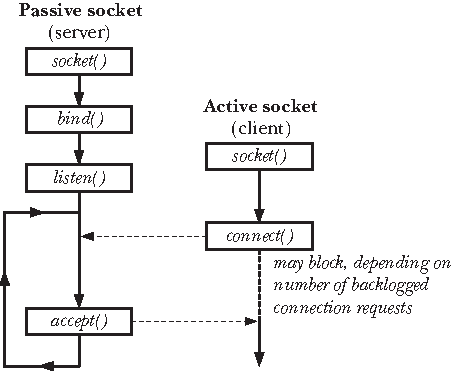
\includegraphics[height = 6cm]{figures/sockets_TCP.pdf}
    % \caption{} % \label{}
\end{figure}
\begin{figure}[H]
    \centering
    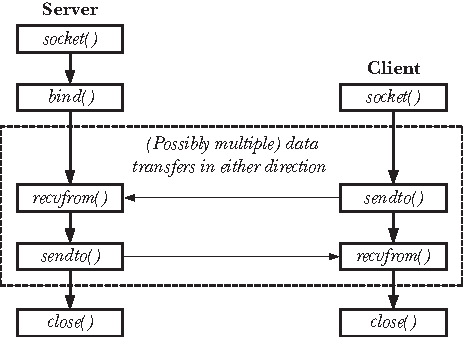
\includegraphics[height = 6cm]{figures/sockets_UDP.pdf}
    % \caption{} % \label{}
\end{figure}
\section{CPU Scheduling}
CPU scheduling is the basis of multiprogrammed operating systems. By
switching the CPU among processes, the operating system can make a
computer more productive. The following sections consider scheduling
algorithms, and the performance metrics used to evaluate them.
\subsection{Basic Concepts}
The objective of multiprogramming is to have a process running at all
times, to maximise CPU utilisation. A process executes until it needs
to wait, typically for an I/O request, entering a waiting queue, so
that another process can be selected for execution. In this model,
several processes are kept in memory, and the CPU is always executing
one of these processes.
\subsubsection{CPU-I/O Burst Cycle}
Process execution consists of a \textbf{cycle} of CPU execution and I/O
wait. A process alternates between these two states until it is
terminated. Process execution begins with a \textbf{CPU burst}, is
followed by an \textbf{I/O burst}, and so on. The duration of each
burst depends on the process and hardware, but generally, \textbf{I/O
bound} processes have short CPU bursts and long I/O bursts, and
\textbf{CPU bound} processes have a few long CPU bursts.
\subsubsection{CPU Scheduler}
The \textbf{CPU scheduler} is responsible for selecting a process from
the \textbf{ready queue} to be executed by the CPU.\@ The ready queue
is a list of processes residing in main memory, waiting to be executed
by the CPU.\@ The ready queue's implementation depends on the
scheduling algorithm used.
\subsubsection{Preemtive and Non-Preemtive Scheduling}
CPU scheduling decisions may take place under the following conditions:
\begin{enumerate}
    \item When processes switch from the running state to the waiting
          state.
    \item When processes switch from the running state to the ready
          state.
    \item When processes switch from the waiting state to the ready
          state.
    \item When a process terminates.
\end{enumerate}
In situations 1 and 4, a new decision must be made, as the current process
cannot continue executing. In situations 2 and 3, a choice can be made
to continue executing the current process, or allow another process to
execute.

When scheduling decisions are made only under conditions 1 and 4, the
scheduling scheme is \textbf{non-preemtive} or \textbf{cooperative}.
When scheduling decisions are made under all four conditions, the
scheduling scheme is \textbf{preemtive} or \textbf{non-cooperative}.

Under non-preemtive scheduling, a process is allocated a CPU, until it
terminates or switches to the waiting state. Under preemtive
scheduling, a condition may cause the currently running process to move
to the ready queue, allowing another process to run.

When using preemtive scheduling it is important to consider access to
shared data and the state of the process when that preemption occurs,
such as when the process is in kernel mode, or if the interrupt occurs
during a critical section.
\subsubsection{Dispatcher}
The \textbf{dispatcher} is the module that gives control of the CPU to
the process selected by the CPU scheduler. This involves:
\begin{itemize}
    \item Switching context from one process to another
    \item Switching to user mode
    \item Jumping to the proper location in the user program to restart
          that program
\end{itemize}
The dispatcher should be as fast as possible, as it is invoked during
every context switch. The time it takes for the dispatcher to stop one
process and start another is known as the \textbf{dispatch latency}.
This is illustrated below
\begin{figure}[H]
    \centering
    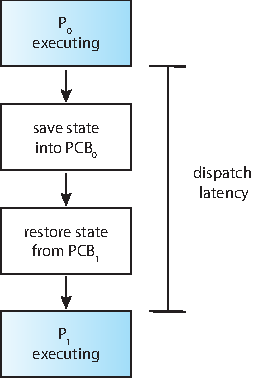
\includegraphics[height = 6cm]{figures/dispatcher.pdf}
    % \caption{} % \label{}
\end{figure}
\subsection{Scheduling Criteria}
The following scheduling criteria are used to evaluate the quality of a
scheduling algorithm:
\begin{itemize}
    \item \textbf{CPU utilisation} --- percentage of time the CPU is
          busy
    \item \textbf{Throughput} --- number of processes that complete
          their execution per time unit
    \item \textbf{Turnaround time} --- amount of time to execute a
          process, from submission to completion
    \item \textbf{Waiting time} --- amount of time a process has been
          waiting in the ready queue after submission
    \item \textbf{Response time} --- amount of time from submission
          until the first response
\end{itemize}
Submission refers to when the process arrives in the ready queue, and
completion refers to when the process terminates or switches to the
waiting queue.
\subsection{Scheduling Algorithms}
\subsubsection{First-Come, First-Served Scheduling}
\textbf{First-come, first-served} (FCFS) scheduling is a non-preemtive
scheduling algorithm that \linebreak schedules processes in the order of arrival.
The implementation of this algorithm is easily managed with a FIFO
queue. When a process enters the ready queue, its PCB is linked onto
the tail of the queue. When the CPU is free, it is allocated to the
process at the head of the queue. The process runs until it terminates
or switches to the waiting state. The CPU is then allocated to the
process at the head of the queue.

The average waiting time for each process in this algorithm varies
significantly based on the arrival order of processes.
\subsubsection{Shortest-Job-First Scheduling}
\textbf{Shortest-job-first} (SJF) scheduling is a non-preemtive
scheduling algorithm that executes processes in order of CPU burst
times. If two processes have the same next CPU burst, FCFS scheduling is
used to break the tie.

SJF scheduling is provably optimal as it yields the minimum average
waiting time, however it cannot be implemented in practise as the
length of the next CPU burst is generally not known in advance.
\subsubsection{Shortest-Remaining-Time-First Scheduling}
\textbf{Shortest-remaining-time-first} (SRTF) scheduling is a preemtive
version of SJF scheduling. When a new process enters the ready queue,
its CPU burst length is compared to the remaining time of the currently
running process. If the new process has a shorter CPU burst, the
currently running process is preempted, and the new process is
allocated the CPU.\@ If the currently running process has a shorter CPU
burst remaining, the new process is added to the ready queue.

Both SJF and SRTF suffer from \textbf{starvation}, where a process with
a long CPU burst may never be allocated the CPU.\@
\subsubsection{Priority Scheduling}
\textbf{Priority scheduling} is a scheduling algorithm that allocates
the CPU to the process with the highest priority. Priority is an integer
value associated with each process, where a low value indicates a high
priority. Priority scheduling may be either preemtive or non-preemtive.

Priority scheduling also suffers from \textbf{starvation}, but can use
\textbf{aging} to prevent this. In aging, as time progresses, the
priority of a ready process increases, preventing low priority
processes from being starved.
\subsubsection{Round-Robin Scheduling}
\textbf{Round-robin} (RR) scheduling is a preemtive scheduling algorithm
that allocates the CPU to each process for a fixed time interval known
as a \textbf{time quantum} or \textbf{time slice}. The ready queue is
treated as a circular queue, such that once the running process has
exhausted its time quantum, it is preempted, and added to the tail of
the ready queue. The process at the head of the queue is then allocated
the CPU for the time quantum. The queue is again treated as a FIFO
queue.

Given \(n\) processes with time quantum \(q\), each process is
allocated the CPU for \(1/n\) CPU time of at most \(q\) time units at
once. No process waits for more than \(\left( n-1 \right) q\) time
units.

For large values of \(q\), RR scheduling degenerates to FCFS, and when
\(q\) is too small, the overhead of context switching becomes too
large.
\subsubsection{Multilevel Queue Scheduling}
In both priority and RR scheduling, all processes are placed in a
single queue and may require \(\mathcal{O}\left( n \right)\) time to
search for the next process to execute.\ \textbf{Multilevel queue}
scheduling uses multiple queues to simplify this process, by
distinguishing between various priority levels. As an example,
processes may be divided into the queues shown in the figure below:
\begin{figure}[H]
    \centering
    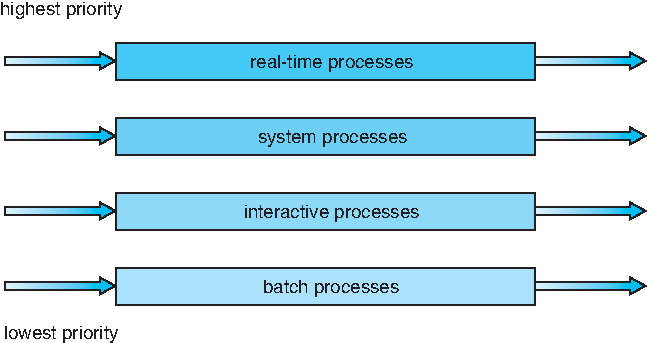
\includegraphics[height = 5cm]{figures/multilevel_queue_scheduling.pdf}
    % \caption{} % \label{}
\end{figure}
A common division is a \textbf{foreground} (interactive) and
\textbf{background} (batch) processes.
In this approach, each queue uses a separate scheduling algorithm, such
as RR for foreground processes and FCFS for background processes.

In addition, there must be scheduling between the queues, which is
commonly implemented as fixed-priority preemtive scheduling. Here, the
higher priority queues are always serviced first, and lower priority
queues are only serviced when higher priority queues are empty. Note
that this has the possibility of starvation.

Alternatively, we can time-slice the queues so that each queue is
allocated a certain amount of CPU time which can be scheduled among its
processes. For example, 80\% of CPU time may be allocated to foreground
processes, and 20\% to background processes.
\subsubsection{Multilevel Feedback Queue Scheduling}
In multilevel queue scheduling, processes are permanently assigned to a
queue when they enter the system. This reduces scheduling overhead, but
is inflexible.\ \textbf{Multilevel feedback queue} scheduling allows
processes to move between queues, by separating processes according to
the characteristics of their CPU bursts. If a process uses too much CPU
time, it is moved to a lower priority queue. Likewise, if a process
waits too long in a lower-priority queue, it may be moved to a
higher-priority queue. This form of aging prevents starvation.

In general, a multilevel feedback queue scheduler is defined by the
following parameters:
\begin{itemize}
    \item The number of queues
    \item The scheduling algorithm for each queue
    \item The method used to determine when to upgrade a process to a
          higher-priority queue
    \item The method used to determine when to demote a process to a
          lower-priority queue
    \item The method used to determine which queue a process will enter
          when that process needs service
\end{itemize}
An example of a multilevel feedback queue scheduler is shown below:
\begin{figure}[H]
    \centering
    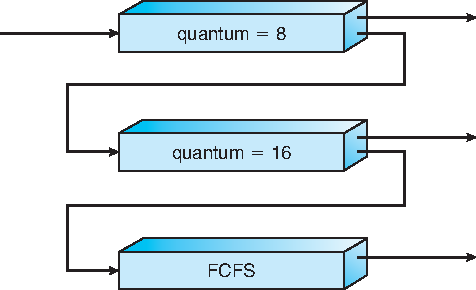
\includegraphics[height = 5cm]{figures/multiple_feedback_queue_scheduling.pdf}
    % \caption{} % \label{}
\end{figure}
\subsection{Thread Scheduling}
On most modern operating systems, kernel-level threads are scheduled
instead of processes. User- level threads are managed by a thread
library and are ultimately mapped to kernel-level threads to be
executed. On systems implementing the many-to-one and many-to-many
models, the thread library schedules user-level threads to run on an
available LWP.\ This scheme is known as \linebreak
\textbf{process-contention scope} (PCS) as competition for the CPU
takes place among threads in the same process. To decide which
kernel-level thread to schedule onto a CPU, the kernel uses
\textbf{system-contention scope} (CSC), where competition takes place
among all threads in the system.
\subsection{Multi-Processor Systems}
Multi-processor systems allow for parallel execution of processes using
load sharing, however this increases the complexity of scheduling. The
term multiprocessor applies to any of the following system
architectures:
\begin{itemize}
    \item Multicore CPUs
    \item Multithreaded cores
    \item NUMA systems
    \item Heteregeneous systems
\end{itemize}
The first three of these architectures have identical or homogeneous
processors.
\subsubsection{Multiple-Processor Scheduling}
One approach to CPU scheduling in a multiprocessor system has all
scheduling decisions, I/O processing, and system activities handled by
a single processor --- the master server. The other processors only
execute user code. This \textbf{asymmetric multiprocessing} is simple
as only one processor accesses the system data structures, reducing the
need for data sharing. A downfall of this approach is that the master
server can become a bottleneck.

Alternatively, each processor may perform its own scheduling, known as
\textbf{symmetric multiprocessing} (SMP). In this approach, each
processor is self-scheduling and processors may either share a common
ready queue, or have their own private queue.

This is illustrated below.
\begin{figure}[H]
    \centering
    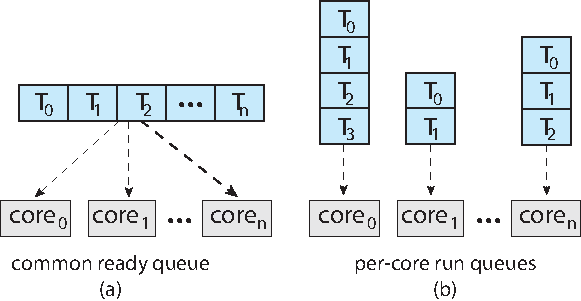
\includegraphics[height = 5cm]{figures/multiprocessor_scheduling.pdf}
    % \caption{} % \label{}
\end{figure}
\subsubsection{Multicore Scheduling}
Multicore processors place multiple CPUs on a single chip to increase
performance and consume less power than multiple single-core
processors. When scheduling on such systems, processes often spend a
significant amount of time waiting for data to become available, as
modern processors operate at much faster speeds than memory. This
situtation is known as a \textbf{memory stall}. Memory stalls may also
be the result of a \textbf{cache miss} (accessing data that is not yet
in the cache).
\begin{figure}[H]
    \centering
    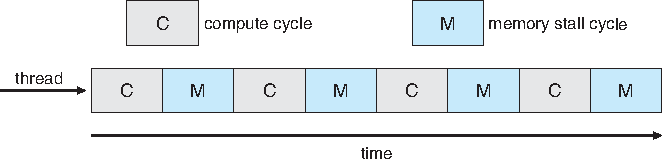
\includegraphics[width = 0.8\linewidth]{figures/memory_stall.pdf}
    % \caption{} % \label{}
\end{figure}
Recent hardware designs implement multithreaded processing cores such
that two (or more) \textbf{hardware threads} are assigned to each core.
By doing so, processors can take advantage of memory stalls by switching
to another thread while waiting for data.
\begin{figure}[H]
    \centering
    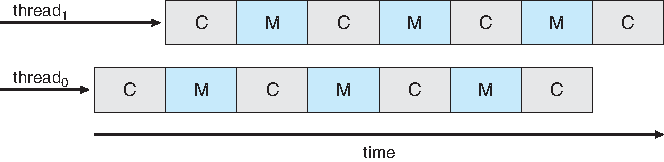
\includegraphics[width = 0.8\linewidth]{figures/memory_stall_2.pdf}
    % \caption{} % \label{}
\end{figure}
\subsubsection{Load Balancing}
On SMP systems, it is important to keep the workload balanced across
all processors to fully utilise the benefits of having more than one
processor.\ \textbf{Load balancing} is the process of redistributing
the workload among the processors.

Load balancing can be implemented in two ways:
\begin{itemize}
    \item \textbf{Push migration} --- a periodic task checks the load on
          each processor and push threads from an overloaded processor to
          idle or less busy processors.
    \item \textbf{Pull migration} --- idle processors pull threads from
          busy processors.
\end{itemize}
\subsubsection{Processor Affinity}
To attempt to keep a thread running on the same processor and take
advantage of a \textit{warm cache}, processes have an affinity for the
processor they are currently running on.\ \textbf{Processor affinity}
is the binding of a process to a particular processor, so that the
process only executes on the designated processor.

Processes may be given one of two types of affinity:
\begin{itemize}
    \item \textbf{Soft affinity} --- the kernel attempts to keep the
          process on the same processor, but may move it to another
          processor for load balancing.
    \item \textbf{Hard affinity} --- the process is bound to a specific
          set of processors, and will not run on any other processor.
\end{itemize}
\section{Deadlocks}
In a multiprogramming environment, several threads may compete for a
finite number of resources. A thread requests a resource, and if it is
not available, enters a waiting state. A \textbf{deadlock} occurs when
a waiting thread cannot change state, because the resource it has
requested is held by other waiting states. The following sections
discuss how to prevent and detect deadlocks.
\subsection{System Model}
A system consists of a finite number of resources to be distributed
among a number of competing threads. Resources are partitioned into
several types, each of which consist of a number of identical
instances. When a thread requests an instance of a resource type, it
may receive any of the available instances of that resource type.

Under normal operation, a thread may utilise a resource in the
following order:
\begin{enumerate}
    \item \textbf{Request} the resource. If the resource cannot be
          granted immediately, it must wait until it can be acquired.
    \item \textbf{Use} the resource
    \item \textbf{Release} the resource
\end{enumerate}
\subsection{Deadlock Characterisation}
A deadlock can arise if four conditions hold simultaneously:
\begin{enumerate}
    \item \textbf{Mutual exclusion} --- at least one resource must be
          held by a single thread.
    \item \textbf{Hold and wait} --- a thread must be holding at least
          one resource, and waiting to acquire additional resources held
          by another thread.
    \item \textbf{No preemption} --- a resource can only be released
          voluntarily by the thread holding it.
    \item \textbf{Circular wait} --- a set of threads must be waiting
          for resources held by each other in a circular manner:
          \(\left\{ T_0,\: T_1,\: \ldots,\: T_n \right\}\) where
          \(T_0\) is waiting for a resource held by \(T_1\), \(T_1\) is
          waiting for a resource held by \(T_2\), and so on, until
          \(T_n\) is waiting for a resource held by \(T_0\).
\end{enumerate}
\subsubsection{Resource-Allocation Graph}
A \textbf{resource-allocation graph} is a directed graph that
illustrates the relationships between threads and resources. This graph
consists of a set of vertices \(V\) and a set of edges \(E\). \(V\) is
partitioned into two different types of vertices:
\begin{itemize}
    \item \(T = \left\{ T_1,\: T_2,\: \ldots,\: T_n \right\}\) for \textbf{threads}.
    \item \(R = \left\{ R_1,\: R_2,\: \ldots,\: R_m \right\}\) for \textbf{resources}.
\end{itemize}
\(E\) consists of two different types of edges:
\begin{itemize}
    \item The directed edge \(T_i \rightarrow R_j\) is known as a
          \textbf{request edge}, and indicates that thread \(T_i\) has
          requested an instance of resource \(R_j\).
    \item The directed edge \(R_j \rightarrow T_i\) is known as an
          \textbf{assignment edge}, and indicates that an instance of
          resource \(R_j\) has been allocated to thread \(T_i\).
\end{itemize}
Graphically, this may be represented by the following shapes:
\begin{itemize}
    \item \textbf{Threads} are represented by circles
    \item \textbf{Resources} are represented by rectangles, with smaller
          squares inside representing available instances of that resource.
    \item \textbf{Request edges} are represented by arrows from a thread to a resource
    \item \textbf{Asignment edges} are represented by arrows from an instance of a
          resource to a thread.
\end{itemize}
When a thread requests an instance of a resource, a request edge is
created from the thread to the resource. When that request is granted,
the edge is converted to an assignment edge (reversed) instantaneously.

From these definitions, it can be shown that if the graph contains on
cycles, then no thread is in a deadlock. If the graph contains a cycle,
then a deadlock may existin one of two possibilities:
\begin{itemize}
    \item if each resource type has exactly one instance, then a cycle
          implies a deadlock.
    \item if each resource type has several instances, then a cycle
          does not necessarily imply a deadlock.
\end{itemize}
The following figure illustrates the graph \(G_1\):
\begin{align*}
    G_1 & = \left( V,\: E \right) = \left( T \cup R,\: E \right) \\
    T   & = \left\{ T_1,\: T_2,\: T_3 \right\}                   \\
    R   & = \left\{ R_1,\: R_2,\: R_3,\: R_4 \right\}            \\
    E   & = \left\{
    T_1 \rightarrow R_1,\: T_2 \rightarrow R_3,\:
    R_1 \rightarrow T_2,\:
    R_2 \rightarrow T_1,\: R_2 \rightarrow T_2,\:
    R_3 \rightarrow T_3
    \right\}
\end{align*}
\begin{figure}[H]
    \centering
    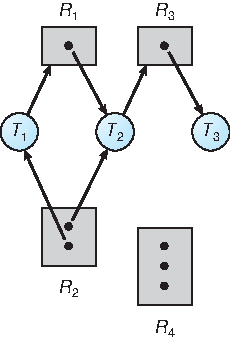
\includegraphics[height = 5cm]{figures/resource_allocation_graph_1.pdf}
    % \caption{} % \label{}
\end{figure}
This graph is not deadlocked as it contains no cycles. Consider the
addition of the directed edge \(R_3 \rightarrow T_2\):
\begin{figure}[H]
    \centering
    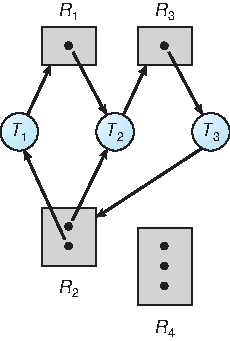
\includegraphics[height = 5cm]{figures/resource_allocation_graph_2.pdf}
    % \caption{} % \label{}
\end{figure}
This edge creates two cycles,
\begin{gather*}
    T_1 \rightarrow R_1 \rightarrow T_2 \rightarrow R_3 \rightarrow T_3 \rightarrow R_2 \rightarrow T_1 \\
    T_2 \rightarrow R_3 \rightarrow T_3 \rightarrow R_2 \rightarrow T_2
\end{gather*}
Further analysis shows that this graph is deadlocked, as each resource
in the cycle is held by a thread waiting for another resource in the
cycle.

The following figure illustrates the graph \(G_2\):
\begin{align*}
    G_2 & = \left( V,\: E \right) = \left( T \cup R,\: E \right) \\
    T   & = \left\{ T_1,\: T_2,\: T_3,\: T_4 \right\}            \\
    R   & = \left\{ R_1,\: R_2 \right\}                          \\
    E   & = \left\{
    T_1 \rightarrow R_1,\: T_3 \rightarrow R_2,\:
    R_1 \rightarrow T_2,\: R_1 \rightarrow T_3,\:
    R_2 \rightarrow T_1,\: R_2 \rightarrow T_4
    \right\}
\end{align*}
\begin{figure}[H]
    \centering
    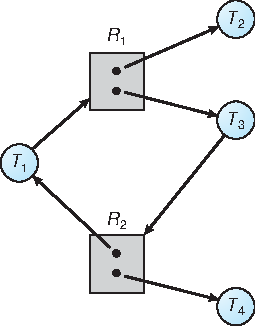
\includegraphics[height = 5cm]{figures/resource_allocation_graph_3.pdf}
    % \caption{} % \label{}
\end{figure}
While this graph contains a cycle, it is not deadlocked as the resources
in the cycle are not held by threads only waiting for other resources
in the cycle. In this case, \(T_2\) and \(T_4\) will eventually release
resources \(R_1\) and \(R_2\) respectively, allowing threads \(T_1\)
and \(T_3\) to acquire the resources they are waiting for.
\subsection{Methods for Handling Deadlocks}
There are three general approaches to handling deadlocks:
\begin{itemize}
    \item Ensure the system never enters the deadlock state
    \item Allow the system to enter the deadlock state, and then
          recover from it
    \item Ignore the problem and pretend that deadlocks never occur in
          the system; used by most operating systems, including Linux
          and Windows
\end{itemize}
\subsection{Deadlock Prevention}
By ensuring at least one of the four necessary conditions for deadlock
cannot hold, deadlocks can be prevented.
\subsubsection{Mutual Exclusion}
Sharable resources such as read-only files do not require
mutual-exclusion and thus cannot be involved in a deadlock. In general,
however, mutual-exclusion cannot be prevented as some resources are
inherently non-sharable. For example, a mutex lock cannot be shared
between multiple threads.
\subsubsection{Hold and Wait}
To prevent the hold-and-wait condition, we must guarantee that when a
thread requests a resource, it is not currently holding another
resource. One way to do this is to require that a thread request all of
its required resources at once, before it begins execution.
Alternatively, we can require that a thread release all of its
resources before requesting any new resources.

Both of these approaches are impractical, as they lead to low resource
utilisation because a resource may be unused for a long period of time,
and starvation if a thread requires multiple resources that are in high
contention by other threads.
\subsubsection{No Preemption}
By allowing preemption, we can prevent the no-preemption condition. If
a thread is holding some resources, and requests another resource that
cannot immediately be allocated to it, then all resources held by that
thread are implicitly released and added to the list of resources that
the thread is requesting. The thread will be restarted only when it
acquires the old resources, and the new resource it is requesting.

This protocol is often applied to resources whose state can be easily
saved and restored, such as CPU registers, but is not practical for
resources such as mutex locks and semaphores.
\subsubsection{Circular Wait}
One way to invalidate the circular-wait condition is to impose a total
ordering of all resource types, and require that each thread requests
resources in an increasing order of enumeration.
\subsection{Deadlock Avoidance}
The above methods for deadlock prevention are often too restrictive,
and thus deadlock avoidance is often used instead. Deadlock avoidance
requires that the system has some additional a priori information about
how resources may be requested by each thread.

One such model requires each thread to declare the \textbf{maximum
number} of resources of each type that it may need. Given this
information, it is possible to construct a \textbf{deadlock-avoidance}
algorithm that dynamically examines the \textbf{resource-allocation
state} to ensure there can never be a circular wait condition. The
resource-allocation state is defined by the number of available and
allocated resources, and the maximum demand of each thread.

Two deadlock-avoidance algorithms are discussed below.
\subsubsection{Safe State}
A system is in \textbf{safe state} if there exists a \textbf{safe
sequence} \(\left( T_1,\: T_2,\: \ldots,\: T_n \right)\) of all threads
in the system such that for each thread \(T_i\), the resources that
\(T_i\) requests can be satisfied by the currently available resources
plus the resources held by all threads \(T_j\) with \(j < i\). When
thread \(T_i\) has finished executing, \(T_{i+1}\) can obtain its
resources, and so on.

If no such sequence exists, the system is in an \textbf{unsafe state}
and a deadlock may occur. Therefore to avoi d deadlocks, a system must
never enter an unsafe state.
\subsubsection{Resource-Allocation-Graph Algorithm}
In a resource-allocation system with only one instance of each resource
type, the resource-allocation graph can be used for deadlock avoidance.
In addition to the request and assignment edges defined before,
consider a \textbf{claim edge} from a thread to a resource. This edge
indicates that the thread \textit{may} request that resource at some
time in the future. On a graph, this is represented as a dashed line.
\begin{itemize}
    \item When a thread requests a resource, a claim edge converts to a
          request edge.
    \item When a thread can be allocated a resource, a request edge
          converts to an assignment edge.
    \item When a thread releases a resource, an assignment edge
          converts to a claim edge.
\end{itemize}
The resource-allocation graph algorithm is as follows:

A request for a resource can be granted only if the resulting
conversion from a request edge to an assignment edge does not contain a
cycle. This can be detected using a cycle-detection algorithm.
\subsubsection{Banker's Algorithm}
In a resource-allocation system with multiple instances of each
resource type, the banker's algorithm can be used for deadlock
avoidance. This algorithm uses several data structures to encode the
state of the resource-allocation system. In a system with \(n\) threads
and \(m\) resource types, the following data structures are used:
\begin{itemize}
    \item \textbf{Available} --- a vector of length \(m\) --- the number of available instances of each resources type.
          \begin{equation*}
              \text{\textbf{Available}}_j = \text{\textbf{Max Available}}_j - \text{\textbf{Allocation}}_j
          \end{equation*}
    \item \textbf{Max} --- an \(n \times m\) matrix --- the maximum
          demand of each thread.
    \item \textbf{Allocation} --- an \(n \times m\) matrix --- the
          number of resources of each type currently allocated to each
          thread.
    \item \textbf{Need} --- an \(n \times m\) matrix --- the remaining
          resource need of each thread.
          \begin{equation*}
              \text{\textbf{Need}}_{ij} = \text{\textbf{Max}}_{ij} - \text{\textbf{Allocation}}_{ij}
          \end{equation*}
\end{itemize}
To determine whether a system is in a safe state, we can use the safety
algorithm:
\begin{enumerate}
    \item Initialise \textbf{Work} and \textbf{Finish}, where
          \textbf{Work} represents the number of available resources of
          each type, and \textbf{Finish} is a vector of length \(n\)
          indicating whether each thread can finish.
          \begin{align*}
              \text{\textbf{Work}}     & \gets \text{\textbf{Available}}                                                 \\
              \text{\textbf{Finish}}_i & \gets \text{false} \quad \forall i \in \left\{ 0,\: 1,\: \ldots,\: n-1 \right\}
          \end{align*}
    \item Loop over \(i\) until no thread can finish:

          If \(\text{\textbf{Finish}}_i = \text{false}\) and
          \(\text{\textbf{Need}}_i \leq \text{\textbf{Work}}\), then
          the thread can finish, and the resources it is allocated are
          released:
          \begin{align*}
              \text{\textbf{Work}}     & \gets \text{\textbf{Work}} + \text{\textbf{Allocation}}_i \\
              \text{\textbf{Finish}}_i & \gets \text{true}
          \end{align*}
    \item If \(\text{\textbf{Finish}}_i = \text{true} \quad \forall i
          \in \left\{ 0,\: 1,\: \ldots,\: n-1 \right\}\), then the
          system is in a safe state.
\end{enumerate}
To determine whether a request for resources can be granted, we can use
the resource-request algorithm:
\begin{enumerate}
    \item If \(\text{\textbf{Request}}_i > \text{\textbf{Need}}_i\),
          then raise an error condition, as the thread has exceeded its
          maximum claim.
    \item If \(\text{\textbf{Request}}_i > \text{\textbf{Available}}\),
          then wait, as the requested resources are not available.
    \item Pretend to allocate the requested resources to the thread by
          modifying the state as follows:
          \begin{align*}
              \text{\textbf{Available}}    & \gets \text{\textbf{Available}} - \text{\textbf{Request}}_i    \\
              \text{\textbf{Allocation}}_i & \gets \text{\textbf{Allocation}}_i + \text{\textbf{Request}}_i \\
              \text{\textbf{Need}}_i       & \gets \text{\textbf{Need}}_i - \text{\textbf{Request}}_i
          \end{align*}
          If the resulting state is safe, the resources are allocated to the thread. Otherwise, the thread must wait for the requested resources,
          and the old resource-allocation state is restored.
\end{enumerate}
\subsection{Deadlock Detection}
If a system does not employ either a deadlock-prevention or
deadlock-avoidance algorithm, then a deadlock may occur. In this case,
the system must provide:
\begin{itemize}
    \item An algorithm that examines the state of the system to
          determine whether a deadlock has occurred
    \item An algorithm to recover from the deadlock
\end{itemize}
Below we discuss two deadlock-detection algorithms for systems with
single and multiple instances of each resource type.
\subsubsection{Single Instance of Each Resource Type}
We define a variant of the resource-allocation graph, that does not
consider resources. This reduces this graph to a \textbf{wait-for}
graph, consisting only of threads and waiting for edges. See (a) and
(b) below:
\begin{figure}[H]
    \centering
    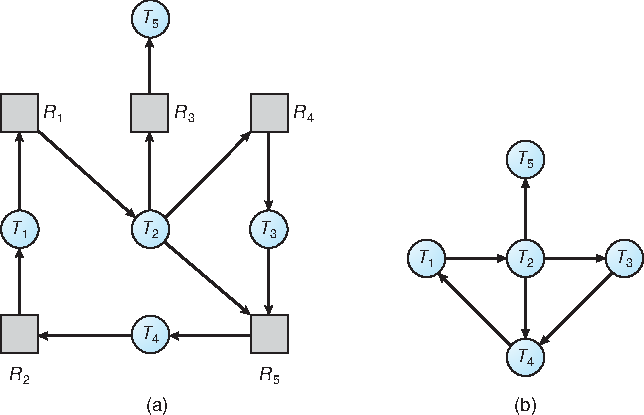
\includegraphics[height = 5cm]{figures/wait_for_graph.pdf}
    % \caption{} % \label{}
\end{figure}
The \textbf{waiting for} edge \(T_i \to T_j\)
indicates that thread \(T_i\) is waiting for thread \(T_j\) to release
a resource. In other words, the resource-allocation graph contains two
edges \(T_i \to R_j\) and \(R_j \to T_i\), for some resource \(R_j\).

In this graph, a deadlock occurs if and only if the graph contains a
cycle. Therefore, the system needs to periodically invoke an algorithm
to detect cycles in the wait-for graph. Such an algorithm requires
\(O\left( n^2 \right)\) time, where \(n\) is the number of threads in
the graph.
\subsubsection{Multiple Instances of Each Resource Type}
When multiple instances of each resource type are available, we can use
data structures similar to the banker's algorithm to detect deadlocks.
The following data structures are used:
\begin{itemize}
    \item \textbf{Available} --- a vector of length \(m\) --- the number of available instances of each resources type.
    \item \textbf{Allocation} --- an \(n \times m\) matrix --- the
          number of resources of each type currently allocated to each
          thread.
    \item \textbf{Request} --- an \(n \times m\) matrix --- the
          number of resources of each type currently requested by each
          thread.
\end{itemize}
The deadlock-detection algorithm is as follows:
\begin{enumerate}
    \item Initialise \textbf{Work} and \textbf{Finish}, where
          \textbf{Work} represents the number of available resources of
          each type, and \textbf{Finish} is a vector of length \(n\)
          indicating whether each thread can finish.
          \begin{align*}
              \text{\textbf{Work}}     & \gets \text{\textbf{Available}}                                                                                                           \\
              \text{\textbf{Finish}}_i & \gets
                                               \begin{cases}
                                                   \text{false} & \text{if } \forall i \in \left\{ 0,\: 1,\: \ldots,\: n-1 \right\} : \text{\textbf{Allocation}}_i \neq \textbf{0} \\
                                                   \text{true}  & \text{otherwise}
                                               \end{cases}
          \end{align*}
    \item Loop over \(i\) until no thread can finish:

          If \(\text{\textbf{Finish}}_i = \text{false}\) and
          \(\text{\textbf{Request}}_i \leq \text{\textbf{Work}}\), then
          the thread can finish, and the resources it is allocated are
          released:
          \begin{align*}
              \text{\textbf{Work}}     & \gets \text{\textbf{Work}} + \text{\textbf{Allocation}}_i \\
              \text{\textbf{Finish}}_i & \gets \text{true}
          \end{align*}
    \item If \(\text{\textbf{Finish}}_i = \text{false}\), then thread
          \(T_i\) is deadlocked.
\end{enumerate}
\subsubsection{Detection-Algorithm Usage}
The frequency of invoking the deadlock-detection algorithm depends on
two factors:
\begin{enumerate}
    \item How often a deadlock is likely to occur
    \item How many threads will be affected by the deadlock---how many
          threads will need to be rolled back (one for each disjoint
          cycle)
\end{enumerate}
Calling a deadlock-detection algorithm too frequently incurs
considerable overhead in computation time, so a less alternative approach
is to simply invoke the algorithm at dfeined defined intervals.

If this detection algorithm is invoked at arbitrary points in time,
then the resource graph may contain many cycles where it will not be
possible to tell which of the many deadlocked threads caused the
deadlock, meaning it will be difficult to recover from the deadlock.
\subsection{Recovery from Deadlock}
When a detection algorithm determines that a deadlock exists, the
system can try to \textbf{recover} from the deadlock automatically.
\subsubsection{Process and Thread Termination}
One way to recover from a deadlock is to abort one or more processes or
threads to break the circular wait condition. This can be done in one
of two ways, each of which reclaims the resources allocated to the
terminated processes or threads:
\begin{itemize}
    \item Abort all deadlocked processes --- this method will clearly
          break the deadlocked cycle, but at the expense of discarding
          all the work done by the aborted processes.
    \item Abort one process at a time until the deadlock cycle is
          eliminated.
\end{itemize}
The order in which processes are aborted may be determined using the following criteria:
\begin{enumerate}
    \item The priority of the process
    \item How long the processes has computed and how much longer it
          will compute before completing its task
    \item How many and what types of resources the process has used
          (are the resources simple to preempt)
    \item How many more resources the process needs to complete
    \item How many processes will need to be terminated
    \item Whether the process interactive or batch
\end{enumerate}
\subsubsection{Resource Preemption}
When preemption is required to eliminate deadlocks, the following
issues must be considered:
\begin{enumerate}
    \item Selecting a victim --- what resources and processes are to be
          preempted. This choice should minimise costs.
    \item Rollback --- after a thread is preempted, resources must be
          reclaimed from the thread, and the thread must be restarted.
          Often this will require the system to keep track of a safe
          state, so that the process is only rolled back as far as is
          necessary.
    \item Starvation --- the same process may be chosen as the victim,
          so we must ensure that a process is preempted a small number
          of times.
\end{enumerate}
\end{document}
